\chapter{Atomes de Rydberg alcalins en interaction}
\label{chapter:Rydberg}
%Atomes de Rydberg : à bas $l$ ou circulaires

Un atome de Rydberg est un atome dont un électron au moins occupe un état de grand nombre quantique principal $n$.
Par là, un atome de Rydberg présente des propriétés physiques exacerbées par rapport à un atome non excité ou peu excité.
On le remarque tout d'abord sur sa taille : un atome de rubidium dans le niveau $n=110$ a une extension spatiale de l'ordre d'$1 ~\si{\micro\meter}$, vingt mille fois plus grande que le rayon de Bohr, qui représente l'ordre de grandeur caractéristique de la taille d'un atome dans son état fondamental.

Avec un électron à une telle distance du c\oe ur atomique, les atomes de Rydberg présentent de très grands moments dipolaires de transition entre états de Rydberg voisins. On comprend dès lors leur très grande sensibilité au rayonnement électromagnétique \cite{ENS_ENHANCED}.
Ces très grands moments dipolaires de transition engendrent également de très forts couplages entre atomes de Rydberg voisins, par l'intermédiaire de l'interaction dipolaire. Ces couplages sont eux aussi plusieurs ordres de grandeur plus importants que ceux qui se manifestent entre des atomes dans le niveau fondamental.
L'interaction dipolaire entre atomes de Rydberg est au c\oe ur des travaux de recherche présentés dans cette thèse. Ce premier chapitre vise à en apporter les éléments théoriques importants pour la compréhension des résultats et discussions qui seront abordés par la suite.

La première partie de ce chapitre décrit la théorie du défaut quantique \cite{TXT_GALLAGHER}, qui permet de calculer les énergies propres des états de Rydberg et leur fonction d'onde radiale loin du c\oe ur atomique positif.
Il est alors aisé de calculer les éléments de matrice de l'opérateur de dipôle électrique entre deux niveaux de Rydberg.
Connaître les dipôles de transition entre un niveau de Rydberg et les niveaux voisins permet entre autres de calculer la durée de vie des niveaux de Rydberg.
Nous introduirons ensuite la base des états paraboliques qui permet une description claire des niveaux de Rydberg circulaires en présence d'un champ extérieur.
La connaissance des dipôles de transition est également essentielle au calcul des interactions dipolaires entre deux atomes de Rydberg, ce que nous aborderons dans un troisième paragraphe.
Enfin, nous discuterons le détail de cette interaction dans deux cas particuliers  : les atomes de Rydberg en interaction autour du niveau $60$S et les atomes de Rydberg en interaction autour du niveau circulaire $50$C.
Ces deux cas particuliers seront à nouveau discutés plus en détail dans des chapitres dédiés aux expériences que nous avons menées.

\section{Les atomes de Rydberg alcalins : des hydrogénoïdes géants}\label{sec:alkalRydberg}
\noindent Un atome de Rydberg alcalin a un seul électron dans un niveau de grand nombre quantique principal $n$. L'essentiel de la fonction d'onde de cet électron est localisé dans des régions atomiques éloignées du c\oe ur, c'est-à-dire de l'ensemble du noyau atomique et des couches électroniques inférieures.
Pour cette raison, il ressemble à un atome d'hydrogène, dont l'unique électron voit un c\oe ur protonique simple de charge totale $+q=\numv{1.602176565(35)d-19}\si{\coulomb}$ \cite{MX_CODATA14}.
Dans le cas de l'hydrogène, ce c\oe ur est plusieurs ordres de grandeurs plus petit que la taille typique de l'orbite de l'électron : le niveau électronique fondamental $1$S a un \og rayon \fg{} caractéristique $a_0 = \numv{0,52917721092(17)}\si{\angstrom}$ \cite{MX_CODATA14}, alors que le proton a un rayon $r_p = \numv{0.8775(51)}\si{\femto\meter}$ \cite{MX_CODATA14}.

Les cinq ordres de grandeur séparant le rayon de l'orbite électronique et le rayon du proton permettent de considérer que le potentiel vu par l'électron est parfaitement coulombien sur tout l'espace.
Les énergies propres de l'atome d'hydrogène sont alors données par
\begin{equation}\label{eq:Hatom}
E(n,l,j)= - \frac{E_I}{n^2} ,
\end{equation}

avec
\begin{equation}\label{eq:E_I}
E_I = \frac{1}{1+\frac{m_e}{M}}\frac{m_e q^4}{32\pi^2 \epsilon _0^2 \hbar ^2}
\end{equation}
l'énergie d'ionisation pour l'électron dans le niveau $1$S de l'atome d'hydrogène, où $M$ est la masse du c\oe ur atomique (masse d'un proton pour l'atome d'hydrogène, masse atomique $m_{Rb87}$ pour l'atome de $^{87}Rb$ dans un état de Rydberg), $n$ le nombre quantique principal, $m_e$ la masse de l'électron, $\epsilon_0$ la permittivité diélectrique du vide, et $\hbar$ la constante de Planck réduite.

Les états propres de ce modèle s'écrivent en coordonnées sphériques comme le produit d'une partie radiale, fonction de $r$ qui est la distance de l'électron au c\oe ur atomique, par une partie angulaire, fonction des coordonnées angulaires $\theta$ et $\phi$ \cite{TXT_COHEN1FR} : 
\begin{equation}\label{eq:Hfonctonde}
\psi(r,\theta,\phi) = R_{nl}(r)\cdot Y_l^{m_l}(\theta,\phi).
\end{equation}
Ici, $l$ est le nombre quantique orbital et $m_l$ le nombre quantique magnétique, associé à la projection du moment angulaire orbital de l'électron sur l'axe de quantification.
Cette première description ne prend pas en compte les corrections aux énergies dues au couplage entre le moment magnétique intrinsèque de l'électron, son spin, et son moment magnétique orbital correspondant à la structure fine.
Elle néglige tout autant le couplage entre le moment magnétique total de l'électron et le moment magnétique du c\oe ur atomique, le couplage hyperfin \cite{TXT_COHEN2FR}.

Là où la structure fine est importante, les bons nombres quantiques deviennent $n,l,j,m_j$, avec $j=l+s$ où $s=1/2$ est le moment magnétique de spin de l'électron. Le couplage hyperfin étant très petit pour les niveaux de Rydberg, nous en ferons fi et continuerons d'utiliser la base avec moment cinétique total $j$ de l'électron pour décrire les niveaux électroniques.

En comparaison avec l'atome d'hydrogène, le c\oe ur positif de l'atome de Rydberg alcalin comporte une structure d'extension spatiale bien plus importante \cite{TXT_GALLAGHER}.
Dans la région des couches électroniques inférieures, le potentiel est bien plus profond que le potentiel coulombien car l'effet d'écrantage partiel de la charge totale positive du c\oe ur par les électrons internes disparaît lorsque l'on s'en approche : c'est l'effet de pénétration du c\oe ur.
Par ailleurs, la distribution spatiale des charges positives et négatives entraîne une polarisabilité du c\oe ur composé.
L'électron de Rydberg interagit avec cette distribution de charge complexe, ce qui modifie sa fonction d'onde et son énergie propre.
Afin de rendre compte de ces effets, il est nécessaire d'apporter une correction aux énergies propres de l'électron de Rydberg d'un atome alcalin : le défaut quantique.

	\subsection{Hamiltonien de l'atome de Rydberg et défaut quantique}
\noindent Les deux effets précédemment cités de pénétration du c\oe ur et de polarisabilité du c\oe ur peuvent être efficacement décrits par la théorie du défaut quantique. Celui-ci apparaît comme une correction $\delta_{nlj}$ au nombre quantique principal $n$ dans l'équation des énergies propres des niveaux électroniques \cite{TXT_GALLAGHER}, qui devient
\begin{equation}\label{eq:E_I_delta}
E(n,l,j) = \frac{- E_I}{(n-\delta_{nlj})^2} ,
\end{equation}
avec 
\begin{equation}\label{eq:deltanlj}
\delta(n,l,j)=\delta_{lj,0} + \frac{\delta_{lj,2}}{(n-\delta_{lj0})^2} + \frac{\delta_{lj,4}}{(n-\delta_{lj0})^4} + \frac{\delta_{lj,6}}{(n-\delta_{lj0})^6} + \cdots .
\end{equation}

\begin{table}[tph!]
	\centering
	\caption[Défauts quantiques du $^{87}Rb$ et $^{85}Rb$]{Défauts quantiques  du \Rb{85} extraits de \cite{MX_GALLAGHERSPECRBNSND03, MX_GALLAGHERSPECRBNF06} et du \Rb{87} extraits de \cite{MX_MACKNSNDRYD}}
	\label{tab:q_defect}
	\begin{tabular}{ c S[table-format=1.12]S[table-format=2.8]  S[table-format=1.10]S[table-format=2.6]}
		\toprule\midrule
		 &  \multicolumn{2}{c}{\Rb{85}}	&   \multicolumn{2}{c}{\Rb{87}}  \\ 
		 \midrule
				  &		$\delta_{lj,0}$				&	$\delta_{lj,2}$		&	$\delta_{lj,0}$			&	$\delta_{lj,2}$ \\ 
		\midrule
		$nS_{1/2}$&  	3.1311804(10)		&	0.1784(6) 	& 3.1311807(8)	& 0.1787(2)	\\
		$nP_{1/2}$&  	2.6548849(10)		&	0.2900(6)	&						&				\\
		$nP_{3/2}$&  	2.6416737(10)		&	0.2950(7)	&						&				\\
		$nD_{3/2}$&  	1.34809171(40)	&	-0.60286(26)&1.3480918(11)	&	-0.6054(4)	\\
		$nD_{5/2}$&  	1.34646572(30)	&	-0.59600(18)&1.3464622(11)	&-0.5940(4)		\\
		$nF_{5/2}$&  	0.0165192(9)		&	-0.085(9)	&						&				\\
		$nF_{7/2}$&  	0.0165437(7)		&	-0.086(7)	&						&				\\
%		$nG$	&0.00400(9)	&&&\\
%		$n,l>4$ & {$0.004(4/l)^5$}&&&\\
		\midrule
		\bottomrule
 	\end{tabular}
\end{table}
%
La série \eqref{eq:deltanlj} développe le défaut quantique en puissances de $1/(n-\delta_{lj,0}) = 1/n^*$ : $n^*$ est le nombre quantique principal corrigé du défaut quantique.
Ses coefficients, présentés en table \eqref{tab:q_defect}, sont extraits des mesures précises des fréquences de transition entre niveaux de Rydberg voisins \cite{ENS_SPECNA2,ENS_SPECCS,MX_MECHEDERYDSPECTRO87} et la série sous cette forme converge rapidement \cite{MX_MARTINSERIESSPECNA} :
pour les niveaux de $n>40$, les deux premiers termes suffisent à obtenir une précision meilleure que la centaine de $\si{\kilo\hertz}$ sur une large gamme de valeurs de $n$.
Les coefficients de la série sont fonction de $l$ et $j$, ainsi que de l'espèce atomique.
Nous n'avons pas connaissance de défauts quantiques mesurés pour le \Rb{87} autres que ceux présentés ici, mais l'utilisation de ceux du \Rb{85} fournit de bons résultats grâce à la grande similarité des structures électroniques de ces deux isotopes.
En ce qui concerne les niveaux de $l>3$, leurs défauts quantiques sont petits, et donc d'autant plus difficiles à mesurer. Ils seront donc négligés par la suite.
Avec les valeurs connues des défauts quantiques, nous obtenons des fréquences de transition entre niveaux de Rydberg voisins avec une précision meilleure que $\sim 50\si{\kilo\hertz}$.

Dans le cas extrême des niveaux de Rydberg circulaires, qui ont un moment orbital maximal $l=n-1$, le défaut quantique peut être considéré nul et alors on retrouve le modèle de l'atome d'hydrogène sans correction autre que la masse du c\oe ur.
		
	\subsection{Partie radiale de la fonction d'onde et calcul du dipôle de transition}
\noindent Ayant ces outils à notre disposition, nous pouvons désormais nous employer à calculer les éléments de matrice de l'opérateur de transition dipolaire $\vec{d}=q\vec{r}$ entre niveaux de Rydberg, qui apparaît de façon essentielle dans les termes de couplage des atomes avec le rayonnement électromagnétique et dans le couplage dipolaire entre deux niveaux de Rydberg $\ket{n,l,j,m_j}$ et $\ket{n',l',j',m_j'}$. Ces éléments de matrice s'écrivent

	\begin{equation}\label{eq:matrixelements}
	\begin{aligned}
	\bra{nl,l,j,m_j}q\vec{r}\ket{n',l',j',m_j'}= & ~q\bra{n,l,j,m_j} r\frac{\vec{r}}{r} \ket{n',l',j',m_j'} \\
	= & ~q\cdot \int r^2dr~R^*_{nl}(r)~r~R_{n',l'}(r)~ \bra{l,j,m_j}\frac{\vec{r}}{r}\ket{l',j',m_j'} \\
	= & ~q.\mathcal{R}(nl,n'l').\mathcal{A}(ljm_j,l'j'm_j')	 ,
	\end{aligned}
	\end{equation}
	
\noindent c'est-à-dire comme produit d'une partie radiale $\mathcal{R}$ et d'une partie angulaire $\mathcal{A}$.
Or la partie radiale $R_{n,l}(r)$ de la fonction d'onde est affectée par l'effet de pénétration du c\oe ur décrit plus haut et doit donc être corrigée \cite{TXT_GALLAGHER}.
Le calcul de $\mathcal{R}$ peut être fait numériquement par une méthode dite de Numerov \cite[pp.10-24]{TXT_GALLAGHER}.
Cette méthode s'appuie sur le fait que le potentiel à l'extérieur du c\oe ur atomique reste coulombien.
La partie radiale de la fonction d'onde peut donc y être calculée à partir de la même équation que pour l'atome d'hydrogène, avec les mêmes conditions aux limites à $r \rightarrow \infty$, mais avec une énergie totale différente qui est fixée par les défauts quantiques, et en tronquant à une distance finie du c\oe ur pour éviter la divergence du potentiel à distance nulle.

\begin{figure}[!h]
	\centering
	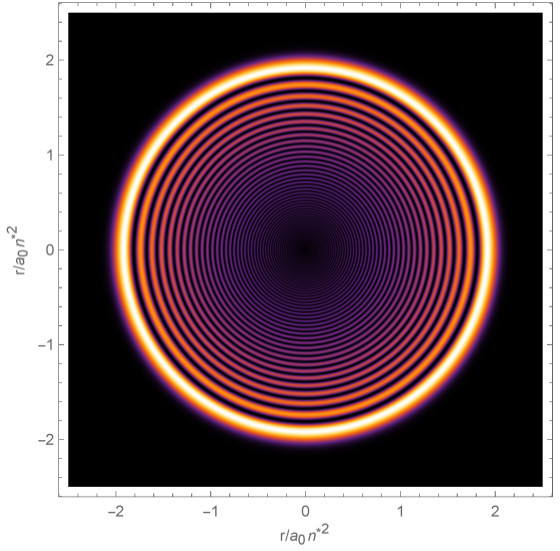
\includegraphics[width=0.6\linewidth]{figures/theory/WaveFunc_60S_}
	\caption[Fonction d'onde du niveau nS]{Probabilité de présence de l'électron dans le niveau nS : $r^2\times |R_{\mathrm{nS}}(r)|^2$, dans l'un quelconque de ses plans de symétrie.}
	\label{fig:wavefunc60S}
\end{figure}

La figure \eqref{fig:wavefunc60S} montre la probabilité de présence $r^2|R_{\mathrm{nS}}(r)|^2$ de l'électron de Rydberg dans le niveau nS du \Rb{87}.
Cela montre que la fonction d'onde se situe essentiellement loin du c\oe ur atomique et justifie donc la validité de la méthode de Numerov.

\`A partir du calcul de $R_{nl}(r)$, l'on peut aisément dériver la partie radiale de l'opérateur dipôle $\vec{d}$.
L'on apprend en particulier que la partie radiale de $\vec{d}$ entre deux niveaux de nombre quantique principal similaire varie comme $\mathcal{R} \sim a_0\cdot n^{*2}$.
Mentionnons ici que le rayon moyen de l'orbitale électronique d'un niveau de Rydberg est très similaire au calcul de la partie radiale de l'opérateur dipôle :
\begin{equation}\label{eq:orbital_size}
\braket{r_{\ket{n,l,j,m_j}}} = \int r^2dr~R_{nl}(r).r.R_{nl}(r) = \mathcal{R}(nl,nl) \propto a_0 \cdot n^{*2}.
\end{equation}
%\`A titre d'exemple, le niveau $60$S a ainsi un rayon moyen de $\braket{r} = 4850~a_0 = \numv{256.5}~\si{\nano\meter}$.
\`A titre d'exemple, l'équation \eqref{eq:orbital_size} permet d'obtenir la taille de l'orbitale électronique dans le niveau $\mathrm{60S_{1/2}}$ : son rayon moyen vaut $\braket{r} = 4850~a_0 = \numv{256.5}\si{\nano\meter}$.

	\subsection{L'effet Stark}\label{sec:Stark}
\noindent Les atomes de Rydberg étant très sensibles au champ électrique, il est important de comprendre comment celui-ci agit.
%Afin de comprendre ce phénomène plus en détail, attardons-nous à décrire l'effet Stark.
La présence d'un champ électrique constant $\vec{F}$ dans l'environnement ajoute au hamiltonien atomique un terme de couplage \og Stark \fg{}  entre le champ et l'opérateur dipolaire électrique.
En présence d'un champ électrique, le hamiltonien devient
\begin{equation}
\label{eq:hamilt_Stark}
\hat{H} = \hat{H}_0 - \vec{\hat{d} \cdot F} = \hat{H}_0 + q~\vec{\hat{r}\cdot F},
\end{equation}
où $\hat{H}_0$ est le hamiltonien libre de l'atome, dont les énergies propres sont calculées par la théorie du défaut quantique selon l'équation \eqref{eq:E_I_delta}, $\hat{\vec{r}}$ l'opérateur position de l'électron dans le potentiel atomique et $q$ la charge élémentaire, supposée positive.

Le hamiltonien Stark \eqref{eq:hamilt_Stark} perd la symétrie sphérique de $\hat{H}_0$, au profit d'une symétrie cylindrique autour de l'axe défini par le vecteur de champ électrique $\vec{F}$.
Cet axe, que nous choisirons comme étant l'axe $(Oz)$, devient alors l'axe de quantification naturel du problème.
Dans la base construite autour de cet axe, le terme d'énergie Stark prend la forme
\begin{equation}
\label{eq:dipole_Stark}
\hat{H}_S = q\hat{z}|\vec{F}| = q\hat{r} \sqrt{\frac{4\pi}{3}} Y_1^0  |\vec{F}|.
\end{equation}
où $\hat{z}$ est la composante selon $z$ de l'opérateur position, $\hat{r}$ sa norme, et $Y_
1^0$ l'harmonique sphérique $(l=1,m_l=0)$.
Ce hamiltonien ne couple que les états de même $m_l$ et vérifiant $\Delta l = \pm 1$.

Le calcul de l'effet Stark par diagonalisation du hamiltonien pour un niveau de Rydberg donné est alors simple à mener numériquement, en réduisant le sous-espace à considérer grâce à la règle de sélection $\Delta m_l = 0$.
Cette même règle de sélection permet d'imposer la condition $\Delta m_j= \Delta m_l + \Delta m_s = 0$, car l'effet Stark n'introduit aucun terme permettant de coupler des états de spins électroniques différents.
La figure \eqref{fig:Stark_60S} montre les énergies propres trouvées par diagonalisation du hamiltonien \eqref{eq:hamilt_Stark}, pour les états d'énergie proche de celle du niveau $\mathrm{60S_{1/2},m_j=1/2}$ et de même $m_j$.
%
\begin{figure}[!h]
\centering
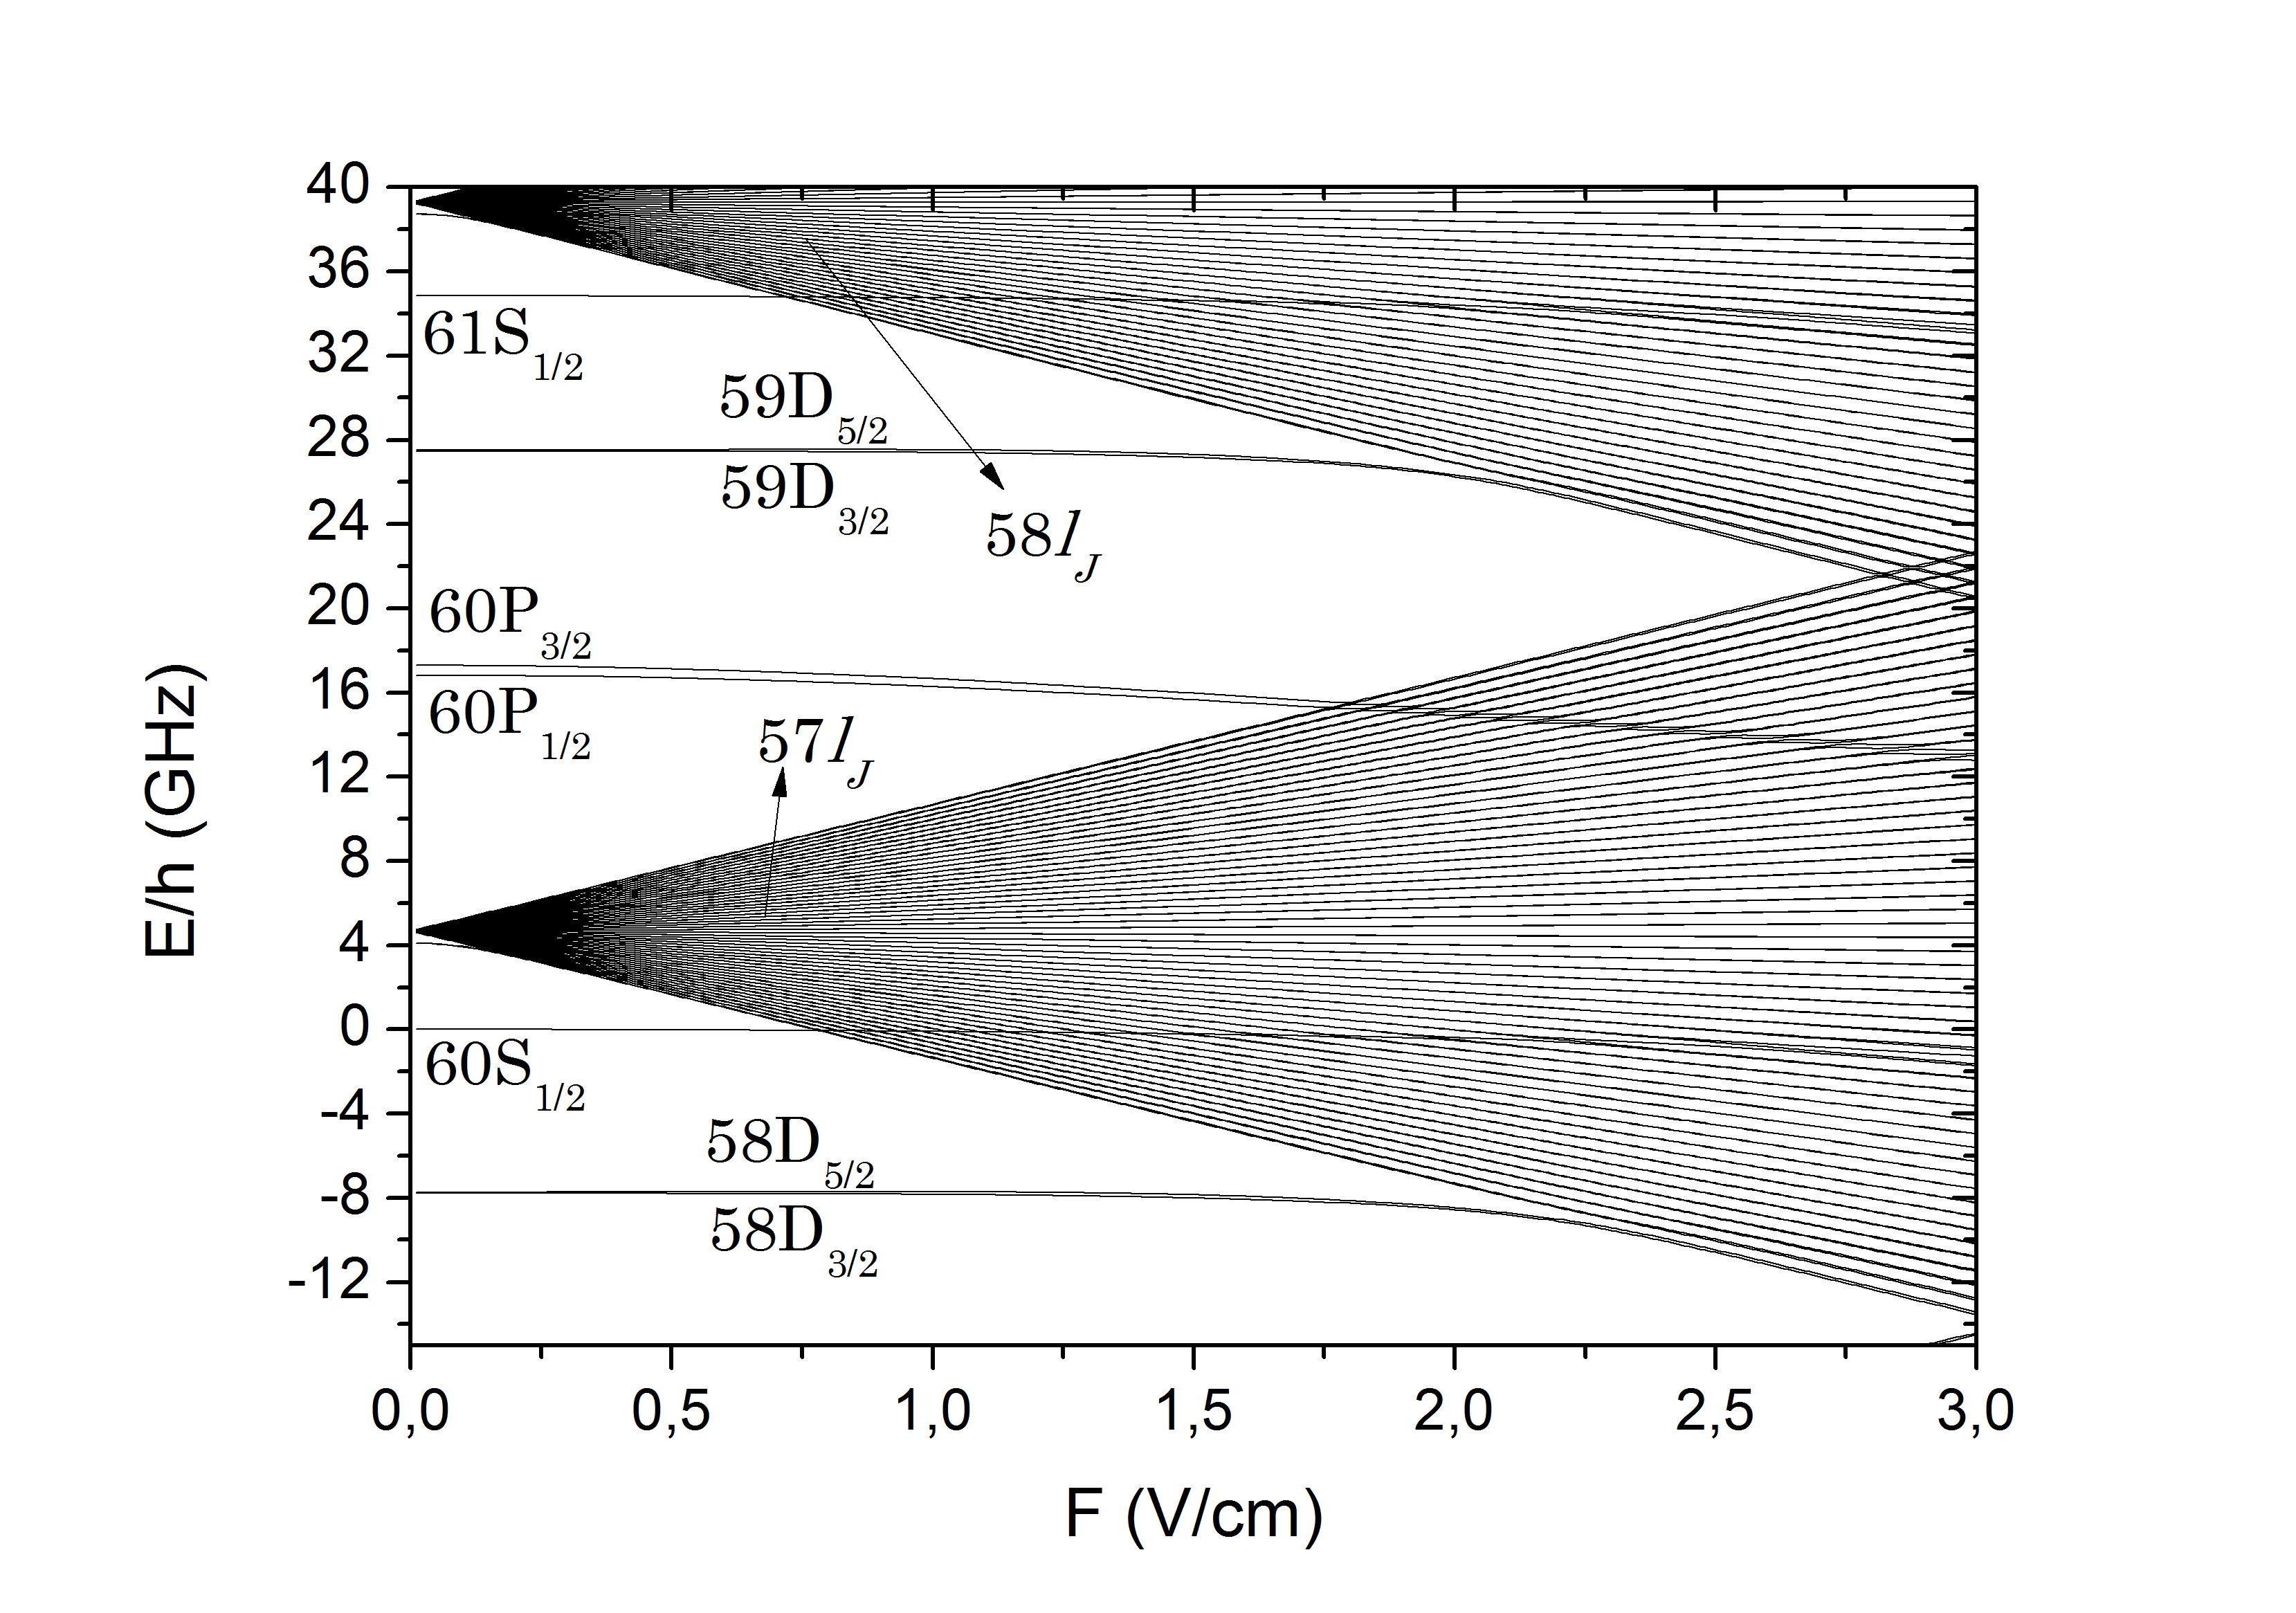
\includegraphics[width=\linewidth]{figures/setup/rydberg/Stark_60S}
\caption[Diagramme Stark autour du niveau $\mathrm{60S}$]{
Diagramme Stark autour du niveau $\mathrm{60S}$, pour les états de $m_j=1/2$.
Le défaut quantique déplace beaucoup les niveaux S,P et D.
Ces niveaux non-dégénérés ont un effet Stark quadratique en champ électrique.
Les niveaux de grand $l$ sont dégénérés et ont un effet Stark linéaire (ce sont les multiplicités qui s'ouvrent en éventail).
}
\label{fig:Stark_60S}
\end{figure}
%
Deux cas sont à distinguer. Les niveaux de faible moment orbital $l\leq 3$ sont déplacés en énergie par leur défaut quantique important.
Le terme d'interaction Stark ne couplant que des niveaux ayant la même énergie en l'absence de champ électrique, ces niveaux S,P et D ne sont perturbés qu'au second ordre par l'effet Stark.
Leur énergie varie donc de façon quadratique avec le champ électrique.
Les niveaux de grand nombre quantique orbital $l$ et de même nombre quantique principal $n$ sont, eux, dégénérés.
Le champ électrique sépare donc leurs énergies linéairement
\footnote{
Le cas de l'effet Stark pour les atomes de grand $l$ sera traité plus en détail dans le chapitre \ref{chapter:circsim}.
}.
La figure \eqref{fig:Stark_60S} montre deux telles multiplicités, $n=57$ et $n=58$.

Les niveaux de bas $l$ présentent donc tous un effet Stark quadratique que l'on exprime sous la forme
\begin{equation}
\label{eq:Stark_quad}
\Delta \nu_S = A\cdot\vec{F}^2.
\end{equation}
%On comprend mieux ainsi la forme des raies présentées en figure \eqref{fig:vieilles_raies} :
%l'effet Stark ne peut que réduire la fréquence de transition $5S-60S$ et la raie n'est donc élargie que du côté des basses fréquences.
%
La diagonalisation du hamiltonien \eqref{eq:hamilt_Stark} et l'ajustement des énergies propres ainsi calculées nous permettent d'extraire les coefficients d'effet Stark pour n'importe quel niveau.
La table \eqref{tab:Stark_60S} répertorie les coefficients d'effet Stark quadratique pour quelques niveaux autour du $\mathrm{60S}$.

\begin{table}[!h]
	\centering
	\caption[Effet Stark quadratique des niveaux proches du $\mathrm{60S}$]{Coefficients d'effet Stark quadratique des niveaux proches du $\mathrm{60S}$.
	}
	\label{tab:Stark_60S}
	\begin{tabular}{c c }
		\toprule\midrule
		Niveau de Rydberg
		& Coefficient Stark quadratique
		\\
		$\ket{n,l,j}$
		& $A_{n,l,j,m_j}$ en $\si{\MHz \per (\V \per\cm) \squared}$ \\
		\midrule
		$\mathrm{60S_{1/2}}$
		& \SI{-89.9}{} \\
		$\mathrm{61S_{1/2}}$
		& \SI{-100.9}{} \\
		$\mathrm{60P_{3/2},m_j=\pm -1/2}$
		& \SI{-676}{} \\
		$\mathrm{60P_{3/2},m_j=\pm -3/2}$
		& \SI{-569}{} \\
		\midrule
		\bottomrule
 	\end{tabular}
\end{table}

%\noindent Si l'on suppose que la largeur des spectres de la figure \eqref{fig:vieilles_raies} est due principalement à l'effet Stark causé par des gradients de champ électrique, alors ceux-ci peuvent s'estimer grâce aux coefficients données en table \eqref{tab:Stark_60S}.
%Une largeur de raie de $\SI{40}{\MHz}$ correspond à un champ électrique variant de $\SIrange{0}{0.667}{\V/\cm}$ sur l'extension du nuage.
%Or le nuage utilisé pour ces spectres était un MOT de $\sim \SI{200}{\um}$ de diamètre, ce qui nous donne une valeur de gradient de champ électrique de l'ordre de $\SI{35}{(\V/\cm)\per\cm}$.

	\subsection{Temps de vie des niveaux de Rydberg}
\noindent Avec la connaissance des dipôles de transition d'un niveau de Rydberg vers les niveaux voisins, 	il est possible de connaître le temps de vie de celui-ci.
Deux processus entrent en jeu dans la désexcitation radiative à température finie de ces niveaux atomiques :
les transitions par émission spontanée mais aussi les transitions par absorption ou émission stimulée par le rayonnement de corps noir de leur environnement.
En effet, les transitions entre niveaux de Rydberg proches en énergie sont dans le domaine des micro-ondes millimétriques.
Cela implique qu'elles seront à considérer dès les très basses températures : contrairement aux photons optiques, des photons micro-ondes sont déjà émis par le rayonnement du corps noir aux températures cryogéniques, de quelques \si{\milli\kelvin} à quelques \si{\kelvin}.

\`A titre d'exemple, la fréquence de la transition entre le niveau $\ket{60\mathrm{S}1/2}$ et le niveau $\ket{59\mathrm{P}3/2}$ vaut $\nu = E/h = \numv{18.5213}\si{\giga\hertz}$. La température de corps noir correspondant à cette fréquence est de $T=h\nu /\kb = \numv{0.89}\si{\kelvin}$.
Cette transition sera donc limitante pour le temps de vie du niveau 60S dès lors que celui-ci sera dans un environnement dépassant les $\numv{500}\si{\milli\kelvin}$.

%Or les températures de rayonnement du corps noir associées à ces gammes de fréquence se situent dans la gamme de quelques \si{\milli\kelvin} à quelques \si{\kelvin}.
\`A température nulle, le temps de vie d'un niveau excité est calculé uniquement à partir des coefficients d'Einstein pour l'émission spontanée \cite{MX_GALLAGHERBBODY}. Un électron dans un niveau excité est couplé aux niveaux de plus basse énergie par les modes électromagnétiques du vide et le taux de désexcitation d'un niveau initial $\ket{i}$ vers un niveau final $\ket{f}$ séparés d'une énergie $E_f - E_i = -\hbar \omega_{if} < 0$ est donné par :
\begin{equation}\label{eq:EinsteinAif}
A_{if} = \frac{2\omega_{if}^3}{3\epsilon_0c^3h}\cdot q^2\cdot |\bra{i}r\ket{f}|^2
\end{equation}
Ce coefficient est le produit de la densité de modes du rayonnement électromagnétique autour de la fréquence résonante $\nu_{if}=\omega_{if}/2\pi$ et du moment dipolaire de transition entre les niveaux $\ket{i}$ et $\ket{f}$ couplés par ce rayonnement.
Le temps de vie de l'état excité est alors calculé en sommant les taux d'émission spontanée vers chacun des niveaux auxquels il a accès par transition dipolaire électrique.
Les transitions dipolaires par émission d'un photon respectant la règle de sélection $\Delta l = \pm1$ et $\Delta m \leq 1$, la quantité de termes à considérer s'en trouve heureusement limitée.

\`A température finie cependant, l'absorption et l'émission stimulée vers les niveaux voisins entrent en jeu.
Le coefficient d'Einstein pour l'absorption et  l'émission stimulée s'écrit ici
\begin{equation}\label{eq:EinsteinBif}
B_{if} = A_{if} . \bar{n}(\omega_{if})
\end{equation}
Il s'agit alors de connaître, pour une température donnée, le taux d'occupation du rayonnement électromagnétique aux fréquences des transitions entre niveaux de Rydberg.
Ce taux nous est donné par la distribution de Bose-Einstein pour un gaz de bosons \cite{TXT_GORECKIPHYSTAT} :
\begin{equation}\label{eq:BoseStat}
\bar{n}(\omega) = \frac{1}{e^{\frac{\hbar\omega}{\kb T}}-1}
\end{equation}
qui devient, lorsque $\kb T \gg \hbar\omega$,
\begin{equation}\label{eq:BoseStat_blackbody}
\bar{n}(\omega) \sim \frac{\kb T}{\hbar\omega}.
\end{equation}
Le nombre de photons par mode varie alors linéairement avec la température et ces photons stimulent des transitions vers des niveaux de Rydberg proches, diminuant ainsi le temps de vie du niveau de départ.


	%\subsection{Le niveau de Rydberg 60S : $\mathbf{\ket{n=60,l=0}}$}
%\noindent Afin d'illustrer les propriétés singulières des niveaux de Rydberg, prenons un exemple qui nous sera utile par la suite : le niveau de Rydberg 60S, qui a donc un moment cinétique orbital $l=0$. Nous nous intéresserons à sa taille, à ses dipôles de transition avec les niveaux voisins, et à son temps de vie.

%Grâce à l'équation \eqref{eq:orbital_size}, nous pouvons obtenir la taille de l'orbitale électronique dans le niveau 60S : son rayon moyen vaut $\braket{r} = 4850~a_0 = \numv{256.5}\si{\nano\meter}$.
%, valeur qui paraît très grande en comparaison avec l'extension spatiale d'un atome dans le niveau fondamental qui est de l'ordre de quelques $a_0$.

\subsubsection*{Temps de vie du niveau $\mathbf{60S_{1/2}}$}
De par la règle de sélection $\Delta l=\pm1$, les termes à considérer pour les transitions dipolaires depuis le niveaux $\ket{n=60,l=0}$ sont les couplages avec les niveaux $n\mathrm{P}_j = \ket{n,l=1,j},~j\in\{1/2,3/2\}$.
La figure \eqref{fig:matrixelements} montre, pour tous les $n$, la somme des coefficients d'Einstein d'émission spontanée et d'absorption et émission stimulée à différentes températures vers les niveaux $n\mathrm{P}_j$.

\begin{figure}[th!]
	\centering
	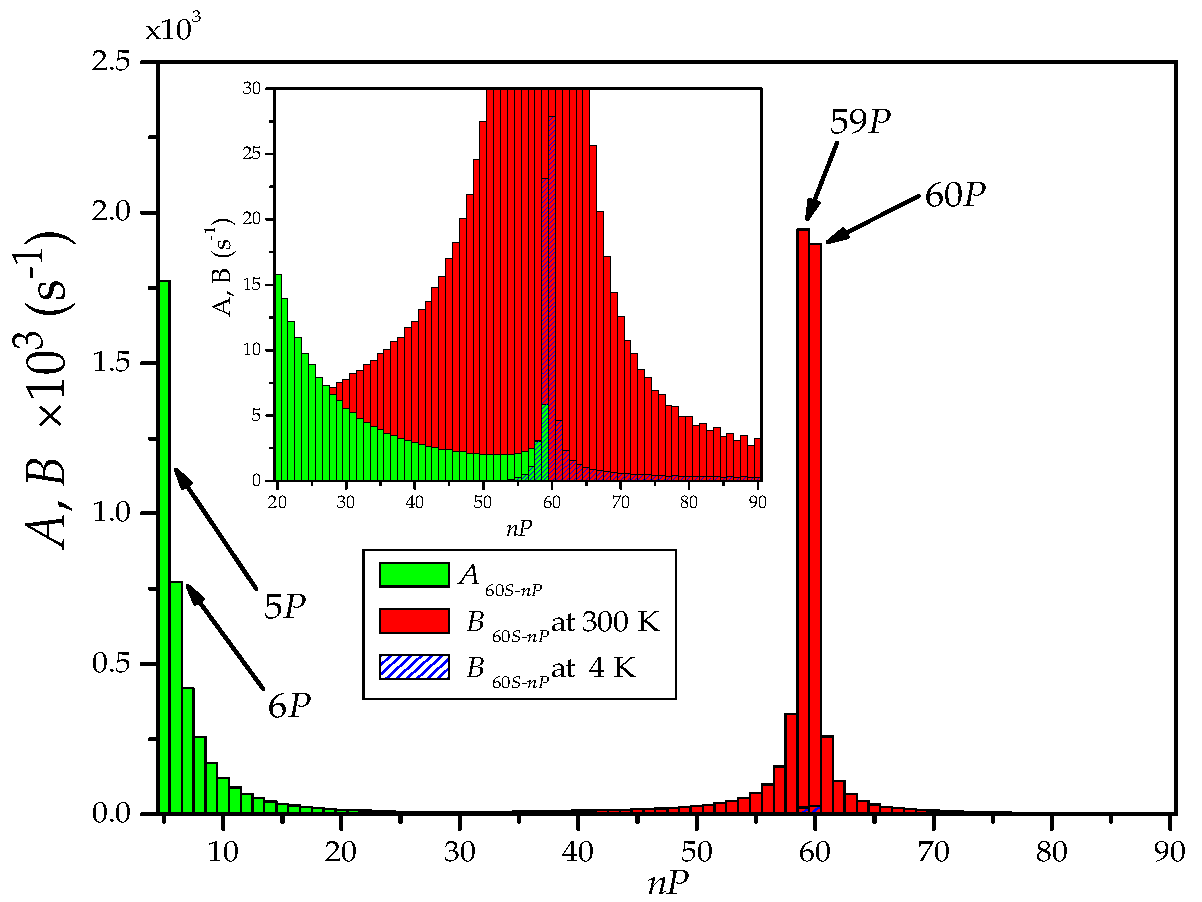
\includegraphics[width=0.7\linewidth]{figures/theory/lifetime}
	\caption[Coefficients d'Einstein de 60S vers $n\mathrm{P}_j,j\in{1/2,3/2}$]{
	Coefficients d'Einstein pour l'émission spontanée (A) et pour l'absorption et émission stimulée par le rayonnement du corps noir(B), depuis le niveau 60S vers les niveaux $n\mathrm{P}_j$.
	Pour chaque $n$, nous montrons la somme des coefficients vers $n\mathrm{P}_{j=1/2}$ et $n\mathrm{P}_{j=3/2}$.
	L'insert montre à une échelle plus adaptée la contribution du rayonnement du corps noir à $\SIv{4}{\kelvin}$.
	}
	\label{fig:matrixelements}
\end{figure}

Il est clair d'après la figure \eqref{fig:matrixelements} que le rayonnement du corps noir à $\numv{4.2}\si{\kelvin}$ contribue peu à une réduction de la durée de vie du niveau 60S par rapport à l'émission spontanée vers les niveaux de bas $n$, alors que le rayonnement du corps noir à $\numv{300}\si{\kelvin}$ aura un effet considérable, ce que confirme la table \eqref{tab:lifetime_60S}.

\begin{table}[h!]
	\centering
	\caption{Temps de vie du niveau 60S à température finie.}
	\label{tab:lifetime_60S}
	\begin{tabular}{c|c c c}
		\toprule\midrule
		\multicolumn{1}{c}{  }
		&\multicolumn{1}{c}{\text{temps de vie à }\numv{0}\si{\kelvin}}
		&\multicolumn{1}{c}{\text{temps de vie à }\numv{4.2}\si{\kelvin}}
		&\multicolumn{1}{c}{\text{temps de vie à }\numv{300}\si{\kelvin}}
		\\ 
		\midrule
		$60\mathrm{S}_{1/2}$
		&$\numv{244.5}\si{\micro\second}$
		&$\numv{239.8}\si{\micro\second}$
		&$\numv{99.4}\si{\micro\second}$\\
		\midrule
		\bottomrule
 	\end{tabular}
\end{table}

Le temps de vie du niveau 60S, de l'ordre de $\SIvv{250}{\us}$ aux températures cryogéniques, permet d'observer et manipuler celui-ci pendant des temps qui sont longs à l'échelle du mouvement d'un nuage de Rydberg.
Cependant si l'on souhaite développer une plateforme de simulation quantique, des temps d'observation beaucoup plus longs sont nécessaires.
Les atomes de Rydberg circulaires ont des durées de vie à température nulle de l'ordre de la dizaine de \si{\ms}, soit cent fois plus que le niveau 60S.
Cela fait des atomes circulaires de bons candidats pour un simulateur quantique.

\section{Les niveaux de Rydberg circulaires}\label{sec:circ_parabol}
\noindent Les niveaux de Rydberg de grand moment orbital, et en particulier les états de Rydberg circulaires, présentent une structure fine et un défaut quantique qui sont très largement négligeables.
Ils sont en cela parfaitement similaires à l'atome d'hydrogène.
On peut utiliser pour les étudier les fonctions d'onde analytiques hydrogénoïdes sans perte de précision.
Pour la même raison, le nombre quantique $j$ qui rend compte du couplage fin n'est plus nécessaire.

Les autres perturbations que peut subir le modèle de l'atome d'hydrogène, comme la présence d'un champ électrique ou magnétique extérieur en deviennent d'autant plus importantes à prendre en compte.
De plus, les niveaux circulaires étant extrêmement anisotropes, l'absence d'axe de quantification leur est préjudiciable.
Ils se mélangent alors rapidement aux niveaux voisins et il est utile de leur imposer un champ électrique, même faible, afin de pallier ce problème.
%En premier lieu, le champ extérieur définit un axe de quantification pour le moment cinétique orbital de l'atome.
%Au cours de ce paragraphe, nous considérerons qu'un axe de quantification est défini selon $(Oz)$ par un champ électrique.
%%, mais nous négligerons pour le moment l'effet Stark, par lequel la présence d'un champ électrique extérieur influence les niveaux électroniques.
%La présence d'un champ selon l'axe privilégié $(Oz)$ brise la symétrie sphérique du problème et la description des fonctions d'onde en coordonnées sphériques, donc sur la base des harmoniques sphériques, n'est plus la mieux adaptée à la situation.

\subsection{La base des états paraboliques}
\noindent	La construction de la base des harmoniques sphériques était fondée sur la conservation du moment cinétique lors du mouvement et sur l'ensemble complet d'opérateurs qui commutent (\og ECOC \fg{}) $\{\hat{H} , \hat{L}^2 , \hat{L}_z \}$
\footnote{
On a ici oublié la structure fine, qui exige lorsqu'elle est prise en compte, de remplacer $\hat{\vec{L}}$ par $\hat{\vec{J}}= \hat{\vec{L}}+\hat{\vec{S}}$.
}.%, où $\hat{J}=\hat{L}+\hat{S}$ est le moment cinétique total de l'électron.
En présence d'un champ électrique extérieur définissant l'axe $(Oz)$, le terme de couplage Stark $-\hat{\vec{d}}\cdot\vec{F} = q\hat{z}|\vec{F}|$ (cf équation \ref{eq:hamilt_Stark}) brise la symétrie sphérique du problème, de façon telle que l'opérateur $\hat{L}^2$ ne commute plus avec le hamiltonien du système.
%Rien ne contrarie cet invariant ici, mais il peut être utile d'en dégager un deuxième.
Il est alors nécessaire de trouver un nouvel invariant du mouvement, qui permettra de définir un nouvel ECOC.
Celui-ci pourra toujours contenir $\hat{L_z}$, qui reste un bon opérateur.

Dès lors que la fonction d'onde électronique reste loin du c\oe ur atomique, l'interaction entre l'électron de valence et le c\oe ur se réduit à un mouvement à force centrale.
La mécanique céleste a traité extensivement des mouvements à force centrale, et nous apprend qu'ils ont en commun l'invariance du vecteur de Runge-Lenz, qui caractérise l'excentricité des trajectoires des corps.
%
L'analogie entre l'interaction gravitationnelle des corps célestes et l'interaction coulombienne au sein des atomes permet de définir l'opérateur vectoriel :
\begin{equation}\label{eq:RungeLenz}
\hat{\vec{A}} = \frac{1}{\sqrt{-2m_e E}} \left( \frac{1}{2} (\hat{\vec{p}}\wedge\hat{\vec{L}} - \hat{\vec{L}}\wedge\hat{\vec{p}}) - m_e e^2 \frac{\vec{r}}{r} \right).
\end{equation}
Cet invariant commute avec le hamiltonien de l'atome d'hydrogène et est de même dimension que l'opérateur de moment orbital $\vec{\hat{L}}$.
Les vecteurs propres de $\hat{\vec{A}}$ prennent donc une forme similaire à ceux de $\hat{\vec{L}}$ et ses valeurs propres varient de $0$ à $\hbar(n-1)$.
%Les relations de commutation des opérateurs $\hat{L}_i$ et $\hat{a}_j$ permettent de construire un opérateur vectoriel $\{\hat{a}_x,\hat{a}_y,\hat{L}_z\}$ vérifiant les relations de commutation d'un moment cinétique :
%\begin{equation} \label{eq:commut_Leta}
%\left\{
%\begin{aligned}
%&[\hat{a}_x,\hat{a}_y]=i\hat{L}_z \\
%&[\hat{a}_y,\hat{L}_z]=i\hat{a}_x \\
%&[\hat{L}_z,\hat{a}_x]=i\hat{a}_y .\\
%\end{aligned}
%\right.
%\end{equation}
%Ce vecteur est donc un générateur des rotations dans l'espace à trois dimensions, défini par les coordonnées $\{ \text{excentricité selon }(Ox), \text{ excentricité selon }(Oy), \text{moment cinétique selon }(Oz)\}$.

Malheureusement, les opérateurs $\hat{\vec{L}}$ et $\hat{\vec{A}}$ ne commutent pas.
Il est donc nécessaire, afin d'obtenir une bonne base de description, de construire de nouveaux opérateurs qui commutent entre eux et vérifient les relations de commutation d'un moment cinétique à trois dimensions.
Les opérateurs
\begin{equation}\label{eq:defJ1J2}
\begin{aligned}
&\hat{\vec{J}}_1 = \frac{1}{2}\left( \hat{L} - \hat{A} \right)\\
\text{et} & \\
&\hat{\vec{J}}_2 = \frac{1}{2}\left( \hat{L} + \hat{A} \right).
\end{aligned}
\end{equation}
vérifient ces propriétés, et commutent avec le hamiltonien.
Au sein d'une même multiplicité, ces opérateurs vérifient 
\begin{equation}\label{eq:defJ1J2sq}
\hat{\vec{J}}_1^2 = \hat{\vec{J}}_2^2 = -\frac{\hbar^2}{4}-\frac{m_ee^4}{8E_n},
\end{equation}
ce qui s'écrit aussi
\begin{equation}\label{eq:E_j1_j2}
E=-\frac{m_ee^4}{2\hbar^2(2j_1+1)^2}=-\frac{m_ee^4}{2\hbar^2(2j_2+1)^2}~.
\end{equation}
L'on retrouve ici le fait que pour une énergie $E$ fixée et donc au sein d'une multiplicité de nombre quantique principal $n$, $\hat{\vec{J}}_1$ et $\hat{\vec{J}}_2$ définissent chacun un moment cinétique $j_{1,2}=(n-1)/2$.

Les états propres au sein d'une même multiplicité sont alors obtenus en diagonalisant $\hat{\vec{J}}_1^2$, $\hat{\vec{J}}_2^2$ et les composantes $\hat{J}_{1z}$ et $\hat{J}_{2z}$.
En notant $\hbar m_{1,2}$ les valeurs propres de $\hat{J}_{1,2~z}$, on pourra caractériser les états propres par les nombres $\{j_1,m_1,j_2,m_2\}$.
Or pour $n$ fixé, $j_1=j_2=(n-1)/2$. Ainsi, un état propre sera entièrement défini par les nombres quantiques $\ket{n,m_1,m_2}$, avec $m_1$ et $m_2$ variant entre $-(n-1)/2$ et $+(n-1)/2$.
Par construction de $\hat{\vec{J}}_{1,2}$, il est aisé de retrouver le nombre quantique magnétique $m=m_1+m_2$.
La figure \eqref{fig:parab_m1m2} propose une représentation schématique des niveaux $\ket{m_1,m_2}$ d'une même multiplicité $n$.

\begin{figure}[!h]
\centering
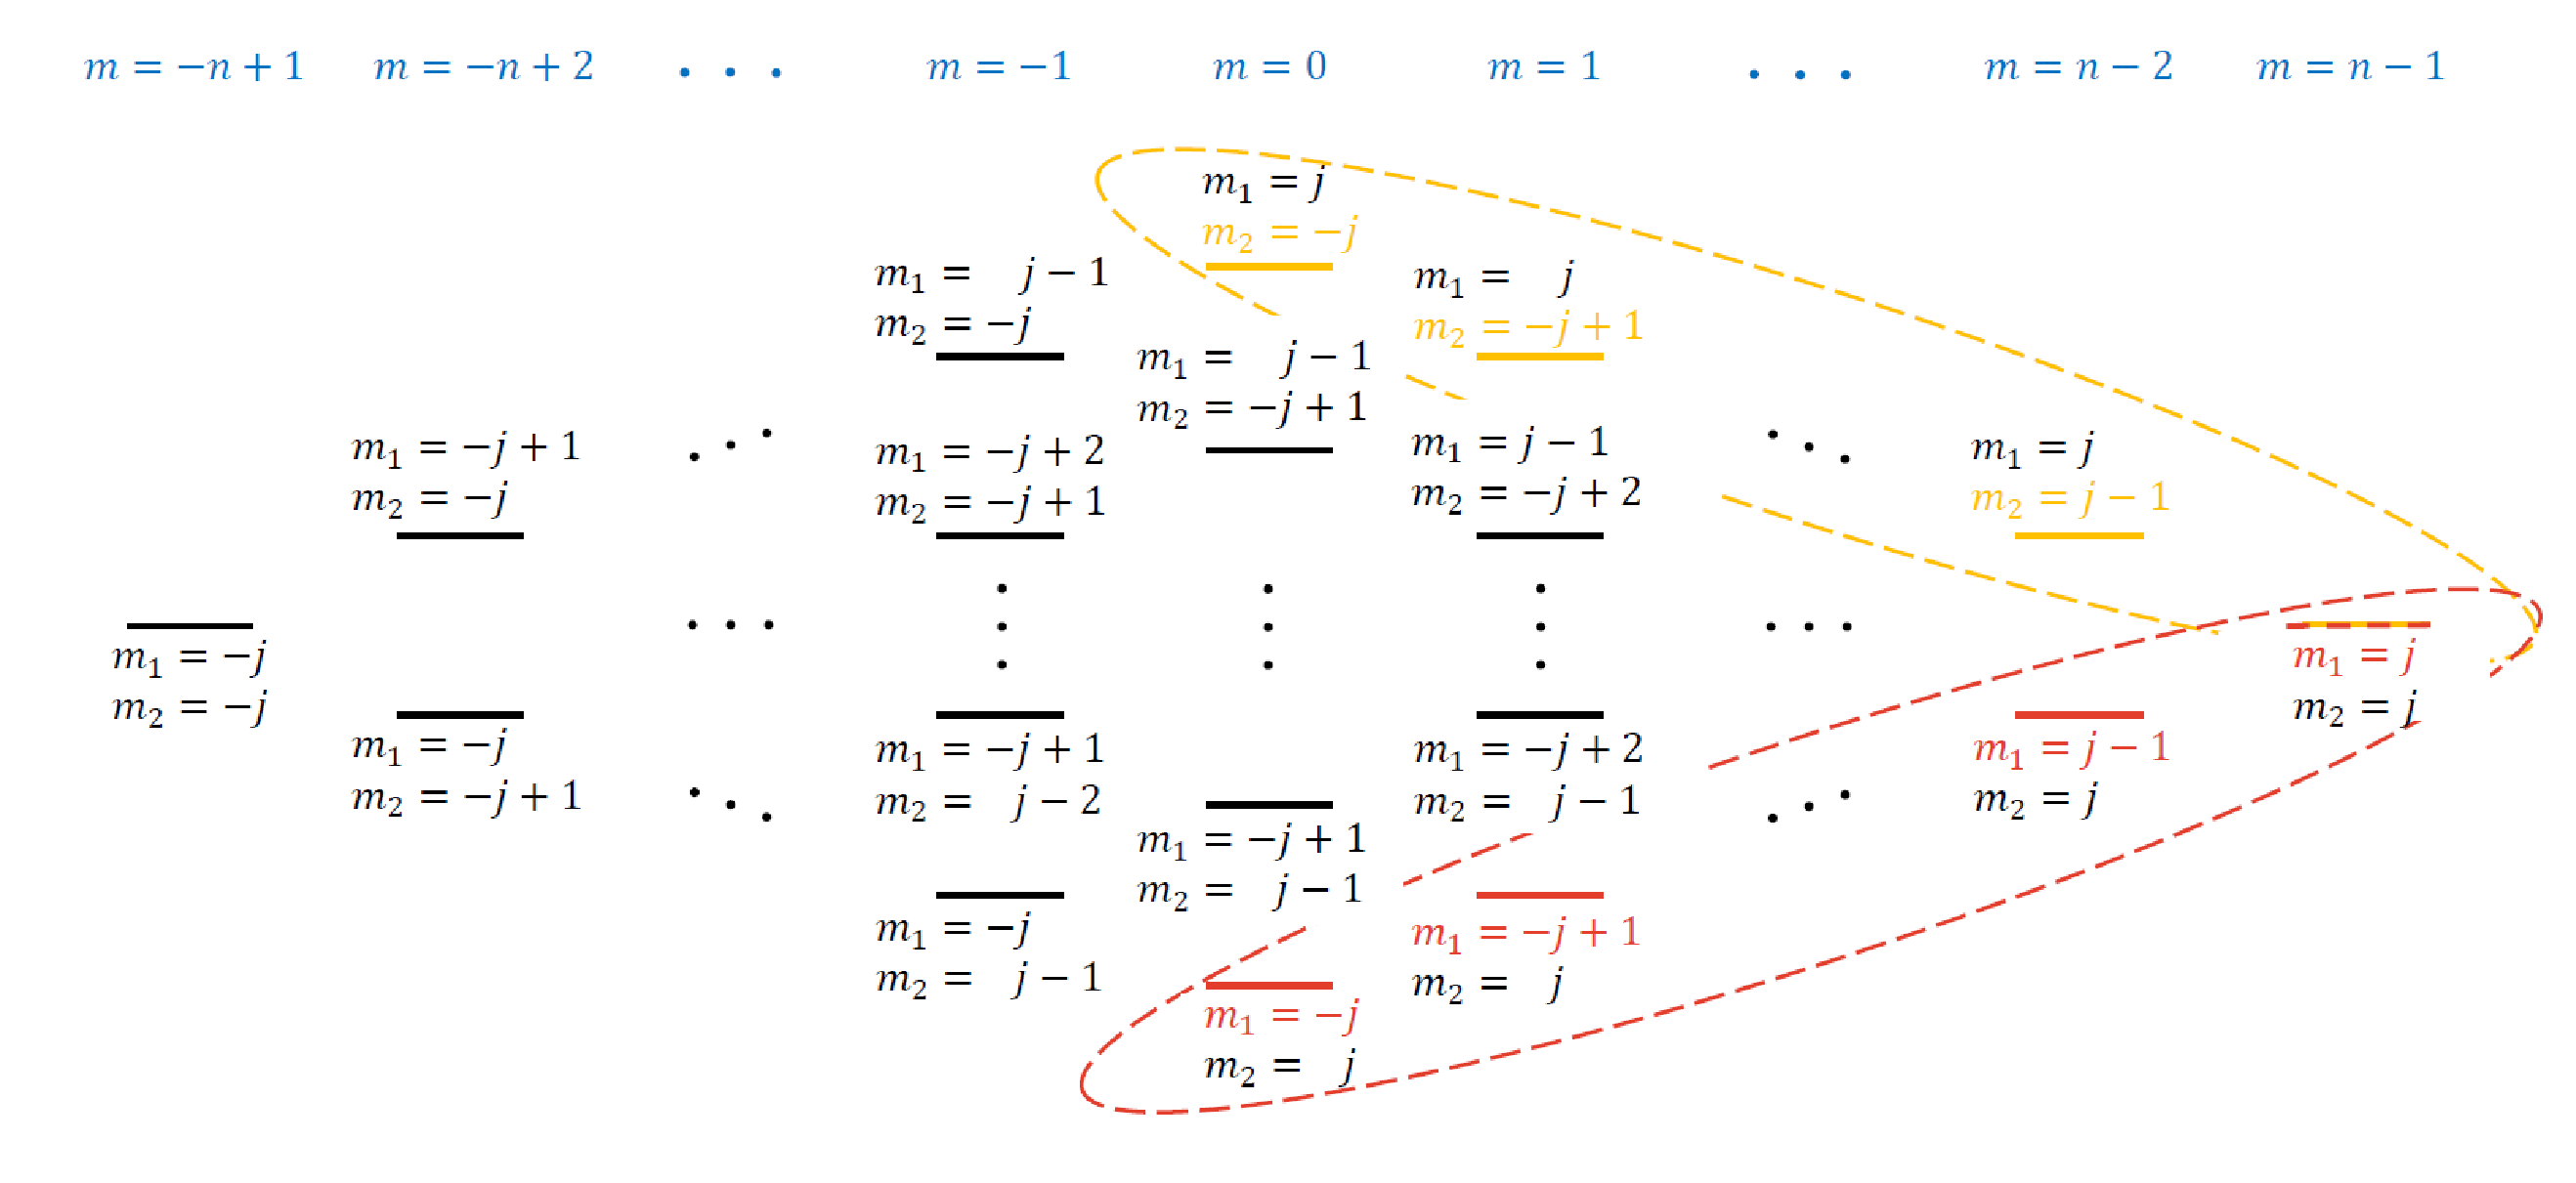
\includegraphics[width=1.\linewidth]{figures/theory/echelle_parabolique_m1m2}
\caption[Échelle des niveaux paraboliques $\ket{n,m_1,m_2}$]{
Niveaux paraboliques $\ket{n,m_1,m_2}$ de même nombre quantique principal $n$, classés horizontalement en fonction de leur nombre quantique magnétique $m=m_1+m_2$. Le nombre $j=j_1=j_2$ est la valeur des moments cinétiques $\hat{\vec{J}}_1$ et $\hat{\vec{J}}_2$ et vaut $j=(n-1)/2$.
La diagonale jaune représente la direction de variation de $m_2$ à $m_1$ fixé et la diagonale rouge la direction de variation de $m_1$ à $m_2$ fixé.
}
\label{fig:parab_m1m2}
\end{figure}


%L'équation de Schrödinger peut s'écrire dans les coordonnées paraboliques $(\xi ,\eta ,\phi )$ obtenues à partir des coordonnées sphériques $(r,\theta ,\phi)$ par la transformation :
%\begin{equation}\label{eq:coordParab}
%\hfill \xi = r(1+\cos\theta) \hfill \eta = r(1-\cos\theta)\hfill
%\end{equation}
%Dans ce système de coordonnées, l'équation de Schrödinger est séparable à condition d'introduire les nombres quantiques $n_1$ et $n2$.
%La base des états paraboliques s'obtient en introduisant les nombres quantiques paraboliques $n_1$ et $n_2$ qui sont fonction de $m_1$ et $m_2$.
%Nous préférerons ici une autre approche pour la plus grande simplicité avec laquelle elle permet de représenter les états atomiques.
%Introduisons à cet effet

Afin d'aider à la représentation des états atomiques, introduisons un nouveau nombre quantique $k=m_1-m_2$, qui quantifie l'excentricité de l'orbite électronique et permet de transformer la base $\ket{n,m_1,m_2}$ en la base $\ket{n,m,k}$ :
\begin{equation}\label{eq:base_nmk}
\left\{
\begin{aligned}
&n \text{ \begin{small}
le nombre quantique principal
\end{small}}\\
&m \text{ \begin{small}
le nombre quantique magnétique variant de
\end{small} }
-(n-1)~~ \text{ \begin{small} à \end{small}} ~~(n-1)\\
&k=m_1-m_2 \text{ \begin{small} variant de\end{small} } (-m-(n-1))~~ \text{ \begin{small} à \end{small} } ~~(-m+n-1).
\end{aligned} \right.
\end{equation}
%


\begin{figure}[!h]
\centering
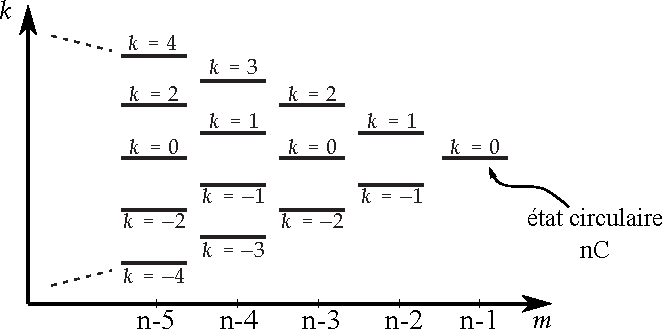
\includegraphics[width=.7\linewidth]{figures/theory/echelle_parabolique_mk}
\caption[Échelle des niveaux paraboliques $\ket{n,m,k}$]{
Niveaux paraboliques $\ket{n,m,k}$ de même nombre quantique principal $n$, classés horizontalement en fonction de leur nombre quantique magnétique $m$ et étiqueté selon le nombre quantique $k$.
Seuls les niveaux de très grand $m$ sont représentés.
}
\label{fig:parab_mk}
\end{figure}

\noindent La figure \eqref{fig:parab_mk} propose une représentation schématique des niveaux $\ket{m,k}$ de $m$ très élevé au sein d'une multiplicité $n$.

Le niveau de $m$ maximal dans une multiplicité donnée, $\ket{n,m=n-1,k=0} =\ket{n,l=n-1,m=l}$, est appelé le niveau circulaire nC.
Sa fonction d'onde électronique se réduit à un tore éloigné du c\oe ur atomique, de rayon $\sim n(n-1)a_0$, et contenu dans le plan perpendiculaire à l'axe de quantification.
La figure \eqref{fig:wavefunc50C} montre la probabilité de présence $r^2|R(r)|^2$ de l'électron dans le plan perpendiculaire à l'axe de quantification, pour le niveau de Rydberg nC. Celle-ci a une présente un rayon moyen valant
\begin{equation}\label{eq:rayon_nC}
\braket{r_{\ket{\mathrm{nC}}}}\simeq  a_0 \cdot n^2.
\end{equation}
Les niveaux de $m$ élevé mais non maximal seront appelés niveaux elliptiques en raison de la forme de leurs fonctions d'onde et seront étiquetés sur la base $\ket{n,m,k}$.
\begin{figure}[!h]
	\centering
	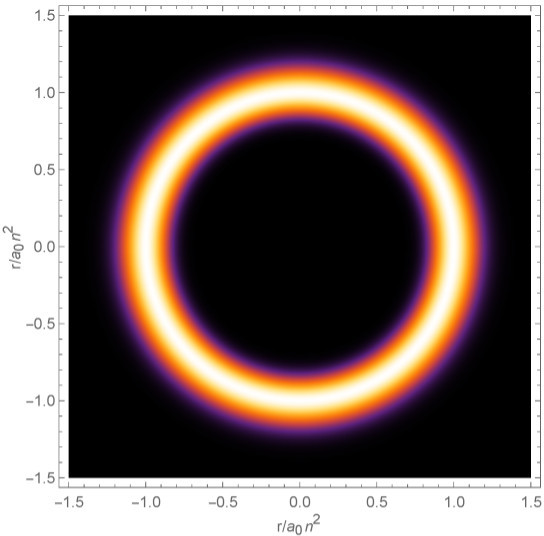
\includegraphics[width=0.5\linewidth]{figures/theory/WaveFunc_50C_}
	\caption[Fonction d'onde du niveau nC]{Probabilité de présence de l'électron dans le niveau nC : $r^2\times |R_{n\mathrm{C}}(r)|^2$, dans le plan perpendiculaire à l'axe de quantification et passant par le noyau.
	Celle-ci décrit un tore de rayon $n^2a_0$ autour du c\oe ur atomique.}
	\label{fig:wavefunc50C}
\end{figure}

%Les circulaires ont besoin d'un champ électrique pour se stabiliser.
\subsubsection*{L'effet Stark pour les atomes de grand moment cinétique}
\noindent Comme nous l'avons dit en \ref{sec:Stark}, dans la base parabolique construite autour de l'axe $(Oz)$ défini par la direction du champ électrique, le terme de couplage Stark prend une forme simple donnée par l'équation \eqref{eq:dipole_Stark} :
\begin{equation}
\label{eq:dipole_Stark2}
\hat{H}_S = q\hat{z}|\vec{F}| = q\hat{r} \sqrt{\frac{4\pi}{3}} Y_1^0  |\vec{F}|.
\end{equation}
%
Dans le cas des niveaux de Rydberg à grand moment cinétique, l'absence de défaut quantique permet de résoudre ce hamiltonien analytiquement par un traitement perturbatif de la forme \cite{TXT_BETHE_ONELECTRONATOMS} 
\begin{equation}
\label{eq:perturbative_energy}
E = E^{(0)}+E^{(1)}+E^{(2)}+\dots,
\end{equation}
où
\begin{equation}
\label{eq:Stark_circular}
\begin{aligned}
&E^{(0)} = -\frac{1}{2n^2} \\
&E^{(1)} = \frac{3}{2}nk|\vec{F}| \\
&E^{(2)} = -\frac{1}{16}\cdot (19+17n^2-9m^2-3k^2) \cdot n^4|\vec{F}|^2.
\end{aligned}
\end{equation}
%
On remarque ici que les états à $k=0$, et en particulier l'état circulaire, ne subissent l'effet Stark qu'au second ordre.

Nous pouvons désormais représenter les niveaux paraboliques $\ket{n,m,k}$ en présence d'un champ électrique qui lève leur dégénérescence.
La figure \ref{fig:parab_mk} se transforme alors en la figure \ref{fig:Stark_nmk}.
%
\begin{figure}[!h]
\centering
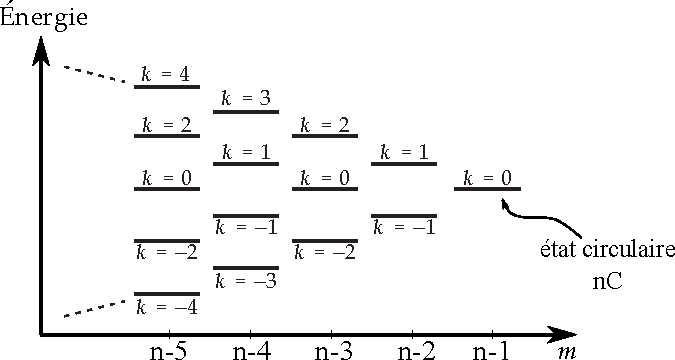
\includegraphics[width=.8\linewidth]{figures/theory/Stark_nmk}
\caption[Échelle des niveaux paraboliques $\ket{n,m,k}$]{
Énergie des niveaux paraboliques $\ket{n,m,k}$ de même nombre quantique principal $n$ en présence d'un champ électrique.
Les niveaux sont classés horizontalement en fonction de leur nombre quantique magnétique $m$ et étiqueté selon le nombre quantique $k$.
Seuls les niveaux de très grand $m$ sont représentés.
}
\label{fig:Stark_nmk}
\end{figure}
%
%Ce diagramme Stark ne ressemble pas à celui des multiplicités $n=57$ et $n=58$ de la figure \eqref{fig:Stark_60S}.
%En effet, ces multiplicités étaient définies non seulement pas leur nombre quantique principal $n$, mais aussi par leur nombre quantique magnétique $m_j = 1/2$.
%Ici au contraire, seul $n$ est fixé.

\subsection{Le niveau de Rydberg 50C : $\mathbf{\ket{n=50,l=49,m_l=49}}$}

\noindent Parmi les niveaux de Rydberg circulaires, le niveau 50C sera d'un intérêt particulier pour nous.
Ce niveau circulaire $n=50$ a une taille valant $\braket{r}_{50C} \simeq 50^2 a_0 = 2500 a_0 = \numv{132}\si{\nano\meter}$.
	

En ce qui concerne leur temps de vie, les niveaux de Rydberg circulaires ont une différence essentielle avec les niveaux de faible $l$ : les niveaux circulaires n'ont de transition dipolaire possible que vers des niveaux eux aussi à très grand $l$, et donc à très grand $n$.
Il n'y a d'ailleurs qu'une seule transition spontanée possible depuis le niveau circulaire $\text{nC}=\ket{n,l=n-1,m_l=l}$, c'est celle vers le niveau circulaire $\text{(n-1)C}=\ket{n'=n-1,l'=n'-1,m_l'=l'}$.
En effet, il n'existe aucun niveau de plus basse énergie que $\mathrm{nC}$ mais qui aurait un $l$ qui lui soit égal ou supérieur.
La figure \eqref{fig:spontem_50C49C} représente les schémas de niveaux près de l'état circulaire $n=50$ et met en évidence l'absence de toute autre transition par émission spontanée depuis le niveau 50C.
Le niveau 50C ne peut donc se désexciter spontanément que vers le niveau 49C, ce qui réduit considérablement la contribution de l'émission spontanée à son taux de désexcitation radiative.
Le calcul du dipôle de transition $\braket{50\text{C}|\hat{\vec{d}}|49\text{C}}$ donne une valeur de $\numv{1704.71} e a_0$.
En appliquant l'équation \eqref{eq:EinsteinAif} à la fréquence de transition $\mathrm{50C}\rightarrow \mathrm{49C}$ de $\SIv{54.25955}{\giga\hertz}$, on obtient un taux de désexcitation valant $\Gamma_{50C}(\SIvv{0}{\kelvin}) = A_{i=50C-f=49C} = \SIv{34.9056}{\hertz}$.
Le temps de vie à température nulle du niveau 50C est donc de $\tau_{0,50C} = \SIv{28.65}{\ms}$, soit cent fois plus que pour le niveau 60S.
\begin{figure}[!h]
	\centering
	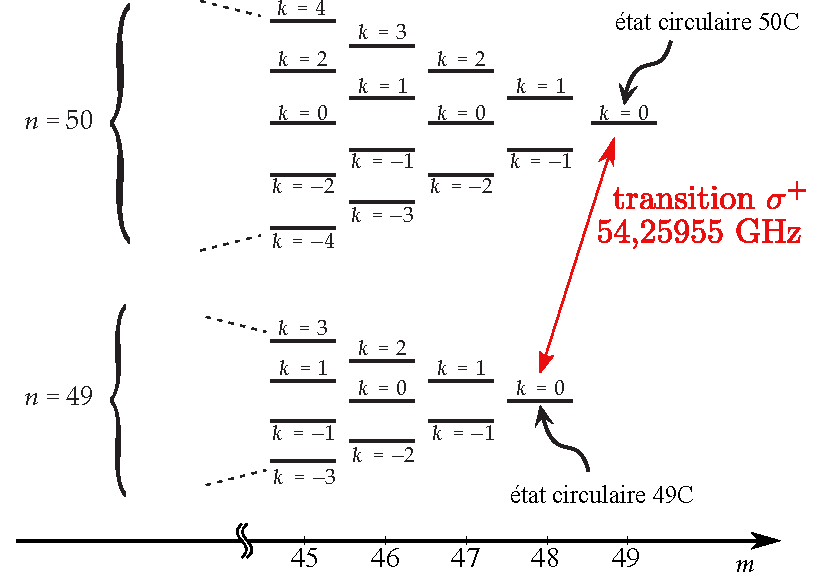
\includegraphics[width=.8\linewidth]{figures/theory/spontem_50C49C}
	\caption[Schéma de niveaux 50C-49C]{Schéma de niveaux des multiplicités $n=50$ et $n=49$ près des niveaux 50C et 49C, en présence d'un champ électrique. La seule transition possible par émission spontanée depuis le 50C est la transition vers le 49C.}
	\label{fig:spontem_50C49C}
\end{figure}

%La limitation de la durée de vie du niveau 50C provient donc en premier lieu de l'absorption et de l'émission stimulée par le rayonnement du corps noir vers les niveaux accessibles par transition dipolaire électrique.
Étant donné le faible taux de désexcitation spontanée du niveau 50C, l'effet du rayonnement du corps noir sur sa durée de vie sera important dès les très basses températures.
Le rayonnement du corps noir amplifiera non seulement le taux de désexcitation vers le niveau 49C, mais autorisera également par absorption les transitions vers les niveaux de $n$ supérieur.
Ainsi, alors que la réduction du temps de vie du niveau 60S entre $\numv{0}\si{\kelvin}$ et $\numv{4.2}\si{\kelvin}$ est faible (voir table \ref{tab:lifetime_60S}, la durée de vie du 60S est réduite de $(1-\numvv{239.8}/\numvv{244.5}) = 2\%$), la réduction du temps de vie du niveau 50C entre $\SIvv{0}{\K}$ et $\SIvv{4.2}{\K}$ est bien plus importante et se porte à $(1-\numv{8.36}/\numv{28.65}) = 71\%$.
\`A température ambiante de $\numv{300}\si{\kelvin}$, la durée de vie de 50C est même réduite à $\numv{122}\si{\micro\second}$, très similaire à celle du niveau 60S.
La figure \eqref{fig:lifetime_50C} montre l'évolution de la durée de vie du niveau 50C en fonction de la température de rayonnement du corps noir, calculée à partir des équations \eqref{eq:EinsteinBif} et \eqref{eq:BoseStat}.


\begin{figure}[!h]
	\centering
	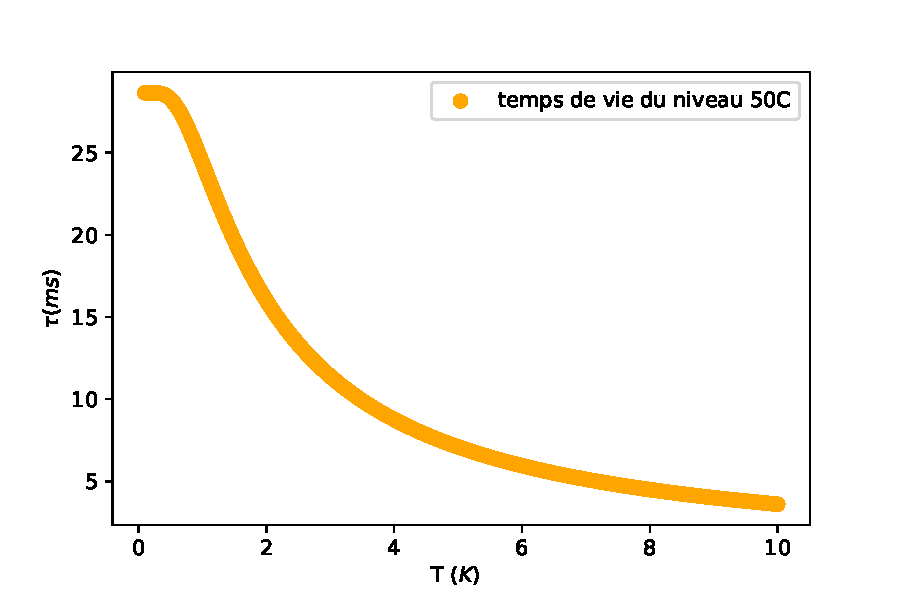
\includegraphics[width=0.8\linewidth]{figures/theory/lifetime_50C}
	\caption[Durée de vie du niveau 50C]{Durée de vie radiative du niveau de Rydberg 50C en fonction de la température de rayonnement du corps noir.}
	\label{fig:lifetime_50C}
\end{figure}

\newpage
Nous avons désormais une bonne connaissance des caractéristiques des atomes de Rydberg individuels, en particulier dans les niveaux 60S et 50C.
Ce sont de très grands atomes, avec de très grands moments dipolaires de transition, et un temps de vie très long.
Comment se comportent ces atomes de Rydberg lorsqu'ils ne sont plus isolés mais proches les uns des autres ?

%\section{Atomes de Rydberg en interaction}
%	\subsection{Deux atomes de Rydberg}
%		\noindent hamiltonien d'interaction entre deux dipôles
%		\[
%		V_{dd} = \frac{1}{4\pi\epsilon_0 r^3} \left( \mathbf{d_1}\cdot \mathbf{d_2} - 3(\mathbf{d_1}\cdot \frac{\mathbf{r}}{r})(\mathbf{d_2}\cdot\frac{\mathbf{r}}{r}) \right)
%		\]
%		\noindent de l'interaction dipole-dipole générale au terme de Van der Waals en $1/r^6$ \\
%		\noindent terme d'énergie et terme d'échange
%	\subsection{les interactions entre Rydberg de bas $l$}
%		\noindent origine du $C_6$ pour 60s-60s et $C_6/A_6$ avec les voisins\\
%		reprendre Raul.figI.3 qui présente la partie radiale du dipôle 60s-ns en fonction de n\\
%		\noindent principe du blocage dipolaire et facilitation (rapide)
%	\subsection{les interactions entre Rydberg circulaires}
%		\noindent $C_6$ pour 50c-50c et $C_6/A_6$ avec les voisins \\
%		\noindent attention à l'anisotropie\\
%		équivalent de la figure ci dessus (Raul.figI.3) pour les 50c, à modifier pour l'anisotropie

\section{Atomes de Rydberg en interaction}\label{sec:interacting_rydbergs}
Dans cette thèse, nous allons nous intéresser aux interactions entre plusieurs atomes de Rydberg voisins, dans des niveaux identiques ou proches en énergie.
Le reste de ce chapitre est consacré au calcul de ces interactions et à leur application aux deux cas qui nous concernent : autour des niveaux 60S et 50C.

	\subsection{Deux atomes de Rydberg qui se parlent}
L'opérateur de moment dipolaire entre deux niveaux de Rydberg proches est grand, comme nous l'avons évoqué.
En cela, les atomes de Rydberg sont de très bonnes antennes pour le rayonnement électromagnétique lorsque celui-ci est résonant avec les fréquences de transition entre niveaux proches.
Cette caractéristique s'accentue fortement lorsque le nombre quantique principal augmente, car le moment dipolaire varie en $n^{*2}$.
Ces grands moments de transition dipolaires font aussi apparaître une interaction importante entre deux atomes de Rydberg différents : bien qu'ils restent des objets neutres électriquement, ces grands dipôles se voient très bien de loin.
En électromagnétisme classique, le terme de couplage entre deux dipôles électriques s'écrit \cite{TXT_JACKSON}
\begin{equation}\label{eq:classicDipole}
V_{dd}(\vec{r}) = \frac{1}{4\pi\epsilon_0 r^3} \left( \vec{d_1}\cdot \vec{d_2} - 3(\vec{d_1}\cdot \frac{\vec{r}}{r})(\vec{d_2}\cdot\frac{\vec{r}}{r}) \right)
\end{equation}
où $\vec{d_1}$ décrit le premier dipôle, $\vec{d_2}$ le deuxième dipôle et $\vec{r}$ le vecteur d'espace qui les sépare.
On peut alors écrire, par analogie, le hamiltonien d'interaction entre deux atomes en remplaçant les dipôles classiques par les opérateurs dipôle électrique de chaque atome.
La distance entre les atomes sera cependant traitée de façon classique, en supposant que la distance entre les atomes est très grande devant l'extension spatiale de leurs fonctions d'onde.
% C'est ce qu'on appelle l'approximation dipolaire. FAUX (commentaire Michel 15 sept
Le potentiel d'interaction dipolaire s'écrit dans ce cas
\begin{equation}\label{eq:quantDipole}
\begin{aligned}
\hat{V}_{dd}(\vec{r}) &= \frac{1}{4\pi\epsilon_0 r^3} \left( \vec{\hat{d}_1}\cdot \vec{\hat{d}_2} - 3(\vec{\hat{d}_1}\cdot \frac{\vec{r}}{r})(\vec{\hat{d}_2}\cdot\frac{\vec{r}}{r}) \right) \\
&= \frac{q^2}{4\pi\epsilon_0 r^3} \left( \vec{\hat{r}_1}\cdot \vec{\hat{r}_2} - 3(\vec{\hat{r}_1}\cdot \frac{\vec{r}}{r})(\vec{\hat{r}_2}\cdot\frac{\vec{r}}{r}) \right).
\end{aligned}
\end{equation}
%
Remarquons que ce terme dépend du produit des opérateurs de transition dipolaire électrique de chaque atome. L'interaction entre atomes de Rydberg varie donc comme $(n^{*2})^2 = n^{*4}$. 

Calculer l'interaction entre deux atomes de Rydberg revient à diagonaliser le hamiltonien total du système des deux atomes dans l'espace de Hilbert des états possibles pour la paire d'atomes.
Sans autre \textit{a priori}, une base naturelle pour cet espace est le produit tensoriel $\ket{R_1}\otimes\ket{R_2}$ des états de chaque atome.
Dans cette base, le hamiltonien du système s'écrit
\begin{equation}\label{eq:hamilt2atoms}
\hat{H} = \hat{H}_{0,1} + \hat{H}_{0,2} + \hat{V}_{dd}(\vec{r})
\end{equation}
où $\hat{H}_{0,i}$ est le hamiltonien de l'atome $i$ isolé.

En l'absence de champ électrique ou magnétique extérieur, l'axe de quantification pour les niveaux de chaque atome n'est pas déterminé.
Il semble naturel de choisir alors comme axe de quantification le vecteur qui sépare les atomes.
Dans cette géométrie, le potentiel d'interaction dipolaire prend la forme
\begin{equation}\label{eq:Vdd_rr1r2}
\begin{aligned}
\hat{V}_{dd}(\vec{r})=&
-\frac{q^2}{4\pi\epsilon_0}\frac{\hat{r}_1\hat{r}_2}{r^3}\frac{4\pi}{3} \times
\left( \hat{Y}^1_1(\theta_1,\phi_1) \hat{Y}^{-1}_1(\theta_2,\phi_2) \right. \\
&\left. + \hat{Y}^{-1}_1(\theta_1,\phi_1) \hat{Y}^{1}_1(\theta_2,\phi_2)
+ 2\hat{Y}^{0}_1(\theta_1,\phi_1) \hat{Y}^{0}_1(\theta_2,\phi_2)
\right)
\end{aligned}
\end{equation}
où les $Y^{m_l}_l$ sont les harmoniques sphériques, solutions des équations de Legendre \cite{TXT_COHEN1FR}.
Dans cette base, l'opérateur $\hat{V}_{dd}$ préserve le nombre quantique magnétique total $M=m_{j1}+m_{j2}$.
Cette condition définit un sous-espace des niveaux de même $M$ pour la paire d'atomes, sous-espace qui a une dimension infinie.
Il sera donc nécessaire, pour calculer l'interaction entre les deux atomes, de tronquer ce sous-espace.
Dans le sous-espace tronqué, nous pouvons diagonaliser le hamiltonien \eqref{eq:hamilt2atoms} pour chaque distance interatomique $r$.

\subsection{Deux atomes dans le même niveau de Rydberg}\label{subsec:interaction_same_level}
Dans le cas de deux atomes dans le même niveau de Rydberg $a$, la règle de sélection $\Delta l = \pm 1$ impose que $\braket{aa|\hat{V}_{dd}|aa} = 0$.
L'opérateur d'interaction dipolaire n'agit donc sur la paire $\ket{aa}$ que comme une perturbation de second ordre, \textit{via} le couplage à des niveaux de paire intermédiaires $\ket{cd}$.
La figure \eqref{fig:Dip_aacd} représente ce couplage au second ordre.
L'énergie d'interaction résultant de cette perturbation prend la forme
\begin{equation}\label{eq:VdW_aacd}
hC_{aa}(r)=\sum_{\ket{cd}}{\frac{\braket{aa|\hat{V}_{dd}|cd}\braket{cd|\hat{V}_{dd}|aa}}{2E_a - E_c - E_d}}  = \frac{hC_{6,aa}}{r^6}
\end{equation}
où $E_i$ est l'énergie d'un atome de Rydberg individuel dans l'état $i$.
L'interaction dipolaire prend donc la forme d'une interaction de Van der Waals en $1/r^6$, avec un coefficient valant $C_{6,aa}$.

\begin{figure}[!h]
\centering

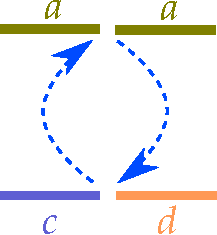
\includegraphics[width=0.3\linewidth]{figures/theory/dipole_coupling_aacd}
\caption[Couplage dipolaire entre mêmes niveaux de Rydberg]{Schéma du couplage dipolaire entre deux atomes dans des niveaux de Rydberg $a$ identiques : le couplage s'effectue au second ordre \textit{via} les niveaux $c$ et $d$.}
\label{fig:Dip_aacd}
\end{figure}

La situation se complique lorsque l'un des niveaux intermédiaires $\ket{cd}$ est quasi-dégénéré avec le niveau $\ket{aa}$, c'est-à-dire lorsque $\braket{aa|\hat{V}_{dd}|cd} \gg |2E_a-E_c-E_d|$.
Le développement perturbatif est en effet invalidé sous cette condition et il est nécessaire de traiter le problème différemment.
Si $\ket{c}=\ket{d}$, alors le sous-espace à observer est composé des deux états $\ket{aa}$ et $\ket{cc}$ et l'on a $E_c\simeq E_a$.
Le hamiltonien d'interaction s'écrit alors
\begin{equation}\label{eq:forster_aacc}
H_{aa-cc} = \bordermatrix{~ 	&\ket{aa} 	& \ket{cc} \cr
	\ket{aa}		&2E_a 		& \frac{\Braket{aa|V_{dd}|cc}}{r^3}	\cr 
	\ket{cc} 		& \frac{\Braket{aa|V_{dd}|cc}}{r^3} 		&2E_a\cr} \ .
\end{equation}
%
Les états propres de ce hamiltonien sont les combinaisons symétrique et antisymétrique $(\ket{aa}\pm\ket{cd})/\sqrt{2}$, et présentent les énergies propres
\begin{equation}\label{eq:forster_aacc_energies}
2E_a \pm \Delta E_{dd} = 2E_a \pm\frac{\braket{aa|V_{dd}|cc}}{r^3}= 2E_a \pm\frac{hC_{3,aa}}{r^3}.
\end{equation}

Si, au contraire, $\ket{c}\neq \ket{d}$, on est alors en présence de trois états dégénérés : $\ket{aa}$, $\ket{cd}$ et $\ket{dc}$.
Il est utile de réécrire ceux-ci en combinant $\ket{cd}$ et $\ket{dc}$ symétriquement et anti-symétriquement en $\ket{C}=(\ket{cd}+\ket{dc})/\sqrt{2}$ et $\ket{NC}=(\ket{cd}-\ket{dc})/\sqrt{2}$.
En effet, $\hat{V}_{dd}$ ne couple pas le niveau $\ket{aa}$ avec le niveau $\ket{NC}$.
On peut donc appliquer le traitement réservé jusqu'ici au cas $\ket{c}=\ket{d}$ en remplaçant $\ket{cc}$ par $\ket{C}$.
Nous obtenons donc deux états propres $(\ket{aa}\mp \ket{C})/\sqrt{2}$ avec les énergies
\begin{equation}\label{eq:forster_aacd_energies}
2E_a \pm \Delta E_{dd} = 2E_a \pm\frac{\braket{aa|V_{dd}|C}}{r^3}= 2E_a \pm\frac{\braket{aa|V_{dd}|cd}}{r^3}= 2E_a \pm\frac{hC_{3,aa}}{r^3}.
\end{equation}
Ces cas particuliers sont analogues à ce que l'on appelle dans d'autres contextes les résonances de Förster \cite{MX_BROWAEYSDD14}.

\subsection{Deux atomes dans des niveaux de Rydberg différents}
\label{subsec:interaction_diff_levels}
Intéressons-nous désormais aux interactions entre deux atomes de Rydberg dans les états $a$ et $b$.
Il y a alors deux états de paire dégénérés $\ket{ab}$ et $\ket{ba}$.
De même que précédemment, les termes de couplage $\braket{ab|\hat{V}|ab}=\braket{ba|\hat{V}|ba}$ sont nuls.
L'on peut tout de même introduire un opérateur potentiel effectif $V_{eff}$ pour le système à deux niveaux $\ket{ab}$ et $\ket{ba}$, qui tiendra compte du couplage éventuel au premier ordre entre $\ket{ab}$ et $\ket{ba}$ mais également des couplages de second ordre avec des états intermédiaires.
Les éléments de matrice de $V_{eff}$ sont
%
\begin{equation}\label{eq:Cab_Aab}
\begin{aligned}
&hC_{ab}=\braket{ab|V_{eff}|ab}=\braket{ba|V_{eff}|ba} \\
\text{et} &\\
&hA_{ab}=\braket{ab|V_{eff}|ba}=\braket{ab|V_{eff}|ba}.
\end{aligned}
\end{equation}
%
L'hamiltonien d'interaction s'écrit sous forme matricielle
\begin{equation}\label{eq:MatrixCab_Aab}
V_{eff} = h\cdot \bordermatrix{~ 	&\ket{ab} 	& \ket{ba} \cr
	\ket{ab}		&C_{ab} 		&A_{ab}	\cr 
	\ket{ba} 		&A_{ab} 		&C_{ab} \cr} \ .
\end{equation}
%
Les termes diagonaux de ce hamiltonien représentent l'interaction directe d'un état de paire avec lui-même, qui se calcule donc comme une perturbation de second ordre \textit{via} les niveaux intermédiaires $\ket{cd}$.
Comme c'était le cas pour deux atomes dans le même état de Rydberg, cette interaction prend la forme de Van der Waals avec un coefficient $C_{6,ab}$ :
\begin{equation}\label{eq:VdW_abab}
hC_{ab}(r)=\sum_{\ket{cd}}{\frac{\braket{ab|\hat{V}_{dd}|cd}\braket{cd|\hat{V}_{dd}|ab}}{E_a + E_b - E_c - E_d}}  = \frac{hC_{6,ab}}{r^6}.
\end{equation}

Les termes non-diagonaux $A_{ab}$ correspondent eux à une interaction au cours de laquelle les deux atomes échangent leurs états.
Si la transition $a\rightarrow b$ est autorisée par les règles de sélection dipolaires, alors cette interaction d'échange est un couplage \textit{direct} de $\ket{ab}$ et $\ket{ba}$.
Il varie donc comme un potentiel dipolaire en $1/r^3$.
Dans le cas contraire, l'interaction d'échange sera un couplage dipolaire indirect au second ordre, variant donc en $1/r^6$, voire d'ordre supérieur, comme l'illustre la figure \eqref{fig:Dip_abab}.

\begin{figure}[!h]
\centering
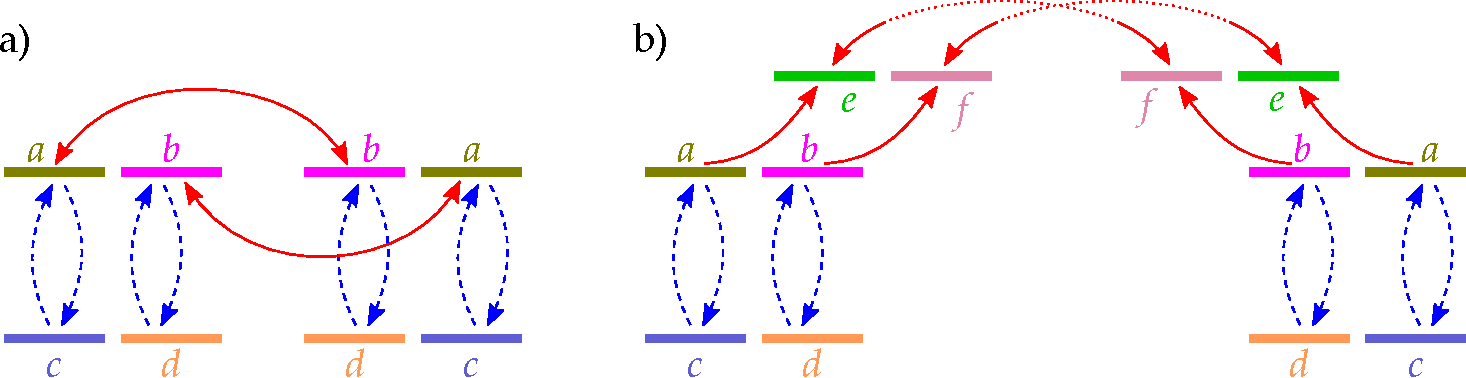
\includegraphics[width=0.9\linewidth]{figures/theory/dipole_coupling_abab}
\caption[Couplage dipolaire entre niveaux de Rydberg différents]{Schéma du couplage dipolaire entre deux atomes dans des niveaux de Rydberg différents $a$ et $b$ : le couplage $ab-ab$ s'effectue au second ordre \textit{via} les niveaux $c$ et $d$. Le couplage $ab-ba$ peut s'effectuer à l'ordre 1(\textbf{a}), à l'ordre 2 via des niveaux intermédiaires $e$ et $f$(\textbf{b}), ou plus encore.}
\label{fig:Dip_abab}
\end{figure}


Lorsque les termes d'échange $A_{ab}$ deviennent comparables aux termes d'interaction directe $C_{ab}$, il peut être judicieux de diagonaliser le hamiltonien effectif \eqref{eq:MatrixCab_Aab}.
En effet, les états propres de celui-ci, qui sont les combinaisons symétrique et anti-symérique $(\ket{ab}\pm \ket{ba})/\sqrt{2}$, ne sont plus dégénérés et présentent respectivement des déplacements d'énergie
\begin{equation}
\label{eq:shift_abab}
\Delta E_{dd} /h = C_{ab} \mp A_{ab}.
\end{equation}

Afin d'illustrer la discussion des interactions que nous venons de présenter, nous allons les appliquer à nos deux exemples que sont le niveau 60S et le niveau 50C.
Dans les deux cas, le calcul numérique consiste à diagonaliser le hamiltonien \eqref{eq:hamilt2atoms} à tous les ordres perturbatifs, en limitant l'espace de Hilbert à quelques centaines d'états de paire et en traitant la distance interatomique de façon classique.

\subsection{Les interactions dipolaires du niveau 60S}

\subsubsection*{L'interaction 60S-60S}
Dans le cas de l'état $\ket{60\text{S},60\text{S}}$, le terme dominant dans la somme \eqref{eq:VdW_aacd} permettant de calculer le coefficient de Van der Waals $C_{6,\text{60S60S}}$ est le coulage avec les paires $\ket{60\text{P}_j,59\text{P}_j}$.
Puisque $E_{60S}-E_{59P}>E_{60P}-E_{60S}$, le dénominateur du terme de couplage principal dans \eqref{eq:VdW_aacd} est positif.
On en déduit que l'interaction 60S-60S, et plus généralement toute interaction dipolaire nS-nS, est toujours répulsive.
%
\begin{figure}[!h]
\centering
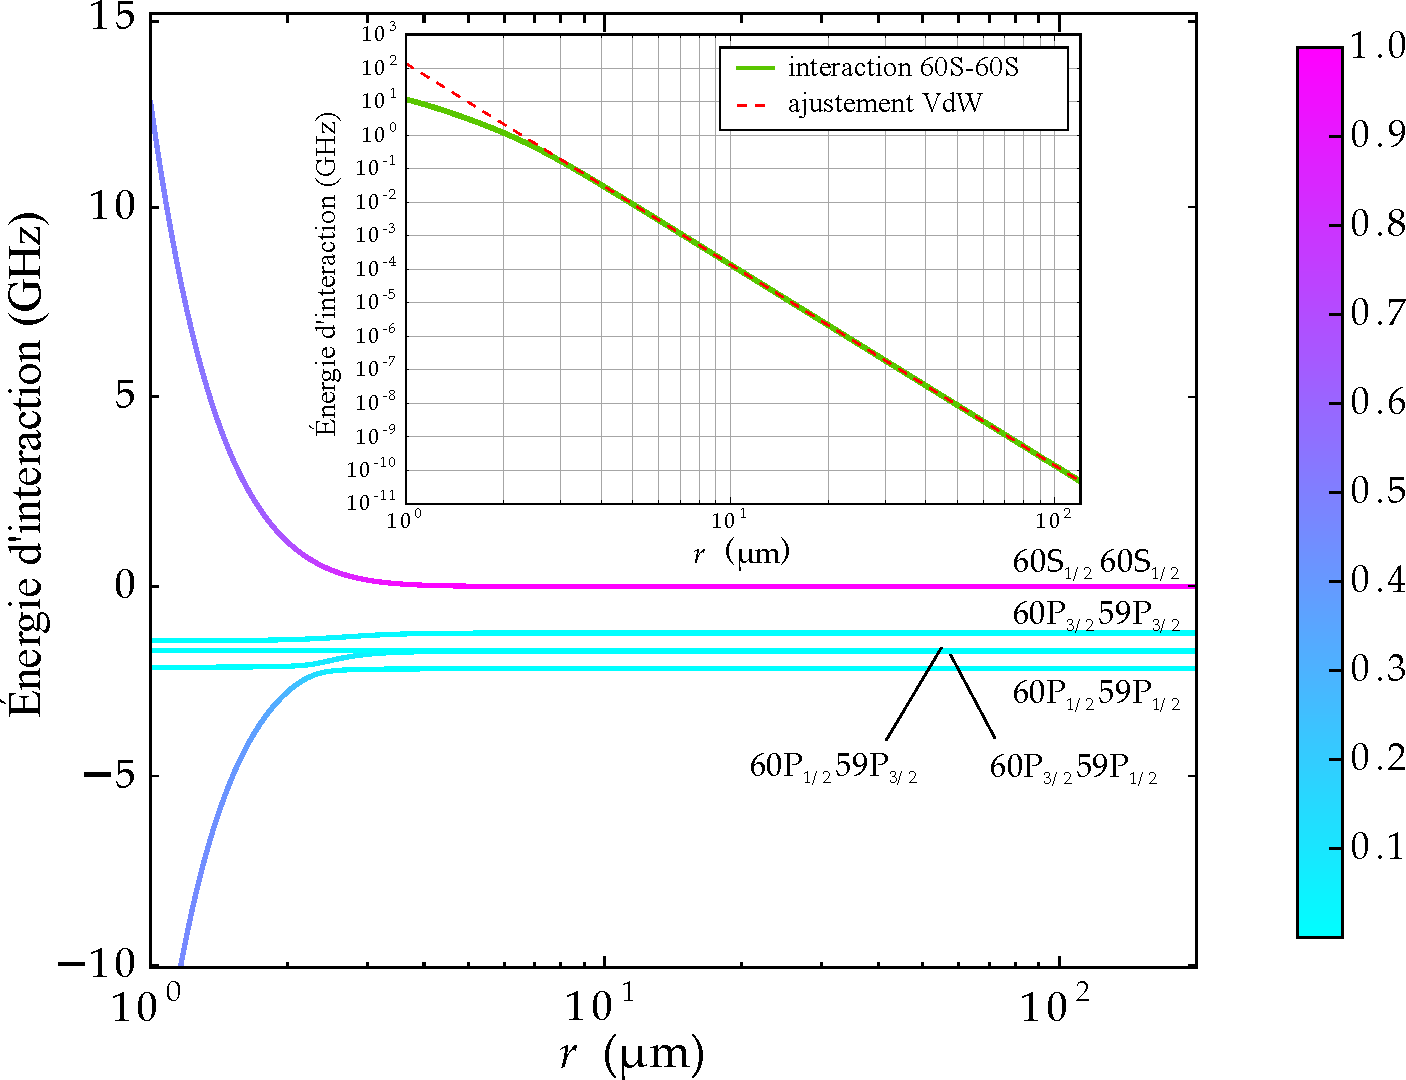
\includegraphics[width=0.8\linewidth]{figures/theory/VdW_60S60S}
\caption[Interaction dipolaire 60S-60S]{Déplacement en énergie de la paire 60S-60S par interaction de Van der Waals. Les différents sous-niveaux $\ket{60\text{P}_j,59\text{P}_j}$ sont représentés. L'échelle de couleur représente le carré de la projection sur l'état non perturbé $\ket{60\text{S},60\text{S}}$.
L'insert représente le déplacement d'énergie en échelle log-log et son ajustement sous la forme de Van der Waals.}
\label{fig:VdW_60s60s}
\end{figure}
%
Le calcul numérique de l'interaction 60S-60S et son ajustement sous la forme de Van der Waals, représentés en figure \eqref{fig:VdW_60s60s}, donnent la valeur
\begin{equation}
\label{eq:C660S}
C_{6,60S60S} = \numv{137.6(1)}\si{\giga\hertz\raiseto{6}\micro\meter}.
\end{equation}

L'ajustement de Van der Waals fonctionne très bien aux distances supérieures à $\sim\SIvv{3}{ \micro\meter}$.
Cependant, aux très courtes distances, la paire $\ket{60\text{S},60\text{S}}$ est très fortement couplée aux niveaux $\ket{60\text{P}_j,59\text{P}_j}$.
La distance critique est celle à laquelle le couplage dipolaire est aussi fort que la différence d'énergie entre les deux états de paire non perturbés, soit ici $\sim \SIv{2}{\giga\hertz}$.
En deçà de cette distance, les états propres du hamiltonien s'éloignent de plus en plus de l'état non perturbé $\ket{60\text{S},60\text{S}}$ et l'interaction évolue vers une interaction dipolaire résonante en $1/r^3$.

\subsubsection*{Les interactions 60S-$nl$}
Le niveau 60S interagit également avec des états de $n$ et $l$ différents.
Il convient alors, comme nous l'avons montré en \eqref{subsec:interaction_diff_levels}, de calculer non seulement les coefficients de Van der Waals $C_{ab}$, mais aussi les éléments de matrice d'échange $A_{ab}$.
De plus, il est possible ici d'avoir des termes d'échange dûs à un couplage dipolaire direct et qui varient donc en $r^3$.

\begin{figure}[!h]
\centering
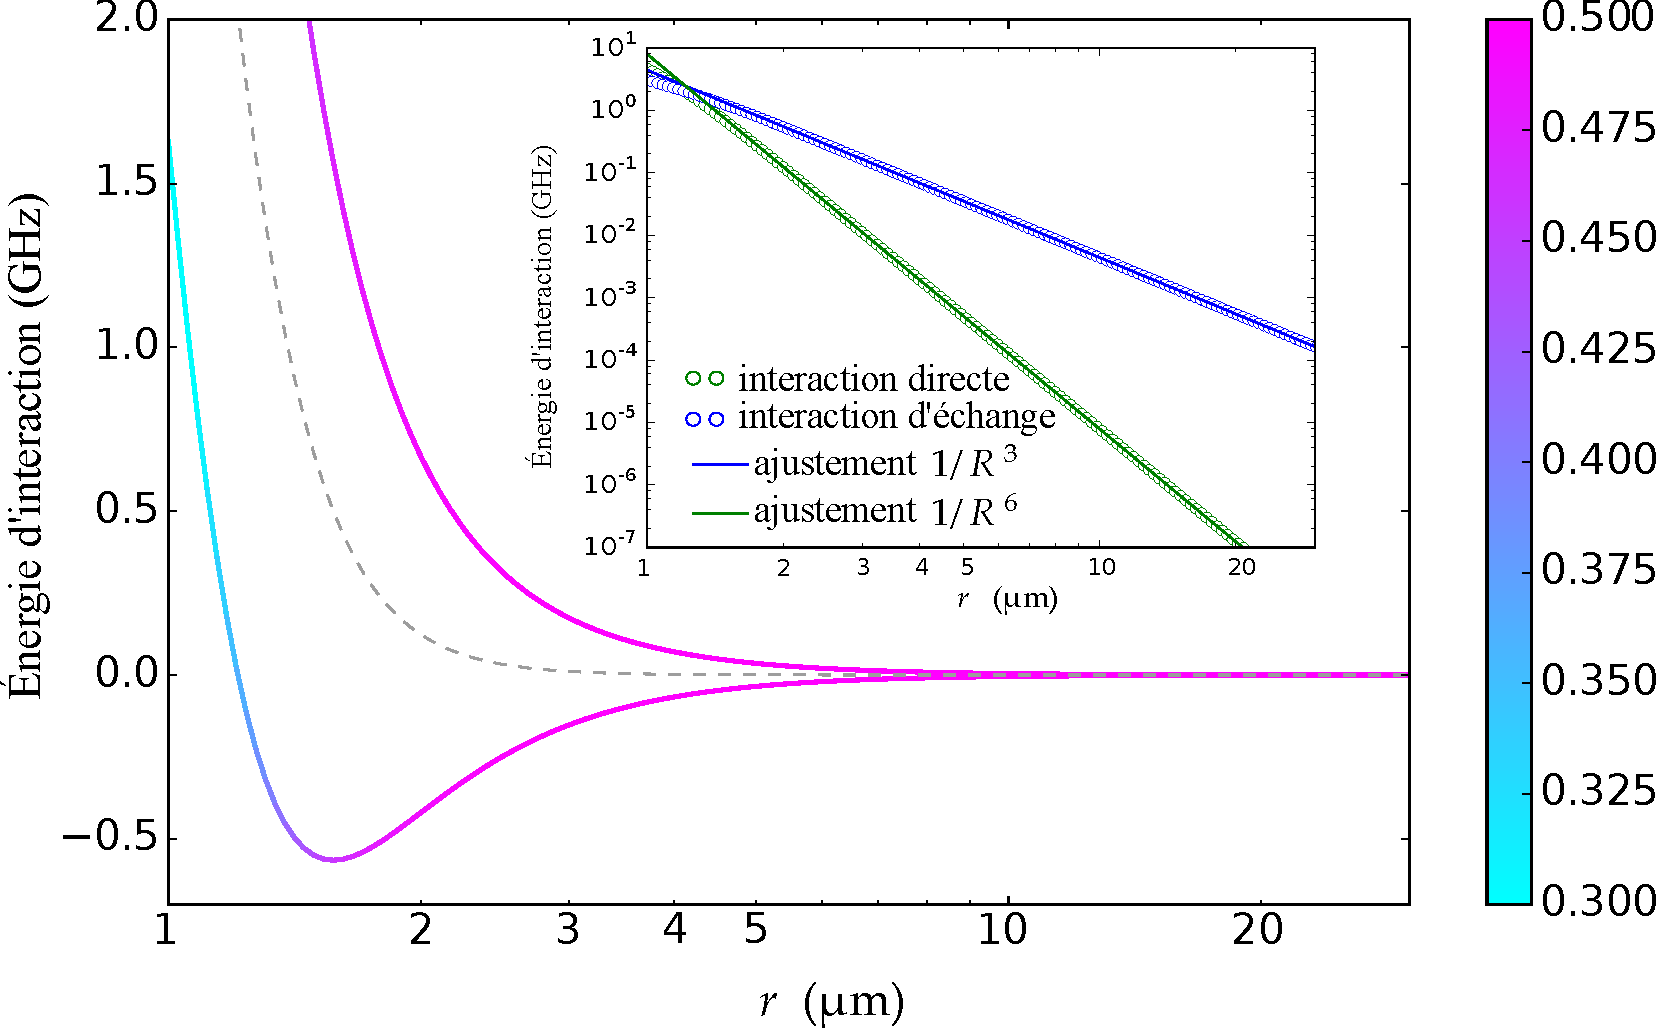
\includegraphics[width=0.8\linewidth]{figures/theory/VdW_60S60P}
\caption[Interaction dipolaire 60S-60P$_{3/2}$]{Énergie de la paire 60S-60P$_{3/2}$ en présence de l'interaction dipolaire.
Les branches inférieure et supérieure correspondent respectivement aux superpositions symétrique et antisymétrique des deux niveaux de départ.
L'échelle de couleur représente le carré de la projection sur l'état non perturbé $\ket{60\text{S},60\text{P}_{3/2}}$.
La ligne pointillée représente le déplacement en énergie dû à l'interaction directe.
L'insert représente le déplacement d'énergie ainsi que le terme d'échange en échelle log-log et leurs ajustements en $1/r^6$ et $1/r^3$ respectivement.
}
\label{fig:VdW_60S60P}
\end{figure}

La figure \eqref{fig:VdW_60S60P} montre par exemple le résultat du calcul de l'interaction dipolaire pour une paire 60S-60P$_{3/2}$.
Aux grandes distances, l'état de la paire est projeté uniformément sur les deux superpositions symétrique et anti-symétrique.
Aux plus courtes distances cependant, d'autres niveaux contaminent la paire, qui n'est plus dans une superposition de $\ket{60\text{S}}$ et $\ket{60\text{P}_{3/2}}$.

En procédant dela même façon, on peut obtenir les coefficients d'interaction dipolaire pour n'importe quelle paire 60S-$nl$. La table \eqref{tab:VdWcoef_60S_nl} synthétise les résultats des calculs numériques pour plusieurs paires contenant le niveau 60S.

\begin{table}[!h]
	\centering
	\caption[Coefficients de Van der Waals 60S-nl]{Coefficients de Van der Waals pour les interactions de paire entre le niveau 60S et différents niveaux voisins $nl$.}
	\label{tab:VdWcoef_60S_nl}
	\begin{tabular}{c c c c}
		\toprule\midrule
%		\multicolumn{1}{c}{  }
%		&\multicolumn{1}{c}{\text{temps de vie à }\numv{0}\si{\kelvin}}
%		&\multicolumn{1}{c}{\text{temps de vie à }\numv{4.2}\si{\kelvin}}
%		&\multicolumn{1}{c}{\text{temps de vie à }\numv{300}\si{\kelvin}}
%		\\ 
		{ }&$C_6$ (\si{\giga\hertz\raiseto{6}\micro\meter}) & $A_6$ (\si{\giga\hertz\raiseto{6}\micro\meter}) & $A_3$ (\si{\giga\hertz\raiseto{3}\micro\meter})
		\\
		\midrule
		$60\text{S}_{1/2}, 60\text{S}_{1/2}$
		&$\SIv{137.6}{}$
		&$\SIv{0}{}$
		&$\SIv{0}{}$\\
		$60\text{S}_{1/2}, 57\text{S}_{1/2}$
		&$\SIv{-43.265}{}$
		&$\SIv{0.325}{}$
		&$\SIv{0}{}$\\
		$60\text{S}_{1/2}, 61\text{S}_{1/2}$
		&$\SIv{290.125}{}$
		&$\SIv{246.475}{}$
		&$\SIv{0}{}$\\
		$60\text{S}_{1/2}, 60\text{P}_{3/2}$
		&$\SIv{7.976}{}$
		&$\SIv{0}{}$
		&$\SIv{4.411}{}$\\
		\midrule
		\bottomrule
 	\end{tabular}
\end{table}



\subsection{Les interactions dipolaires du niveau 50C}
	
\noindent L'interaction dipolaire entre atomes de Rydberg de très grand moment cinétique est rendue plus complexe du fait de leur forte anisotropie.
En effet, l'interaction entre deux dipôles dépend de l'orientation relative de ceux-ci.
Dans le cas des niveaux $l=0$ tel que le 60S, le problème ne se posait pas car ces niveaux sont à symétrie sphérique.
Dès lors que l'on s'intéresse à l'interaction entre des niveaux à symétrie cylindrique, il est indispensable de savoir comment les atomes s'orientent l'un par rapport à l'autre.
L'interaction dipolaire entre atomes circulaires est encore compliquée par l'introduction d'un champ électrique extérieur, qui déplace et déforme les niveaux par effet Stark.
Le détail de l'interaction dipolaire entre atomes circulaires en présence d'un champ sera discuté au chapitre \ref{chapter:circsim}, mais nous prendrons le temps ici de développer la situation la plus simple :
celle de deux atomes dans le niveau 50C dont les deux orbites sont contenues dans le même plan, comme l'illustre la figure \eqref{fig:double_torus}.
%
\begin{figure}[!h]
\centering
\vspace{1em}
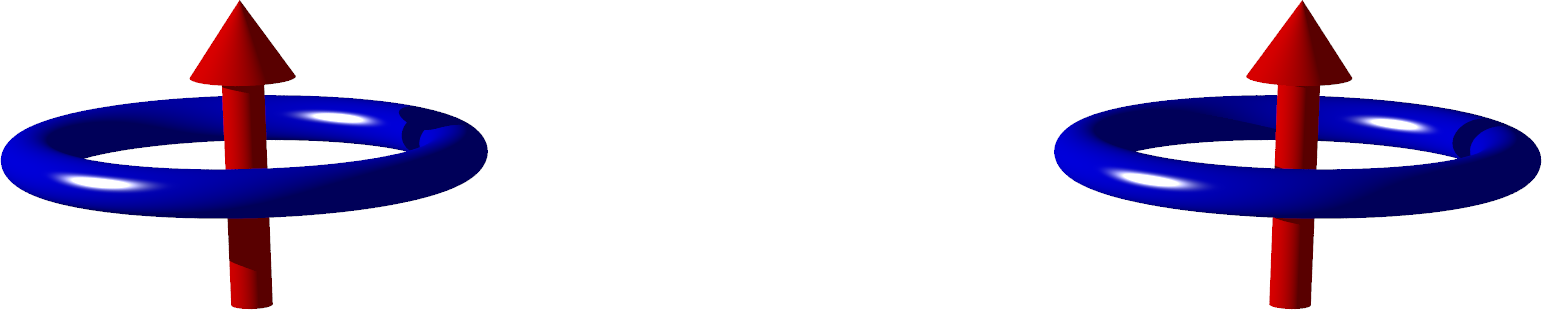
\includegraphics[width=.8\linewidth]{figures/theory/double_torus.png}
\caption[Deux atomes circulaires côte à côte]{Représentation de deux atomes de Rydberg circulaires dont les orbites sont dans le même plan.
Les tores bleus représentent les orbites électroniques et les flèches rouges la direction du moment cinétique.
Si l'on imagine que le dessin est à l'échelle, alors les atomes sont ici séparés d'une distance d'environ \SIv{660}{\nm}.}
\label{fig:double_torus}
\end{figure}
%
Comme il a été dit en \ref{sec:circ_parabol}, les atomes de Rydberg circulaires ont besoin d'un champ électrique extérieur pour se stabiliser.
Nous imposerons donc un champ de \SIvvSym{1}{\V\per\cm}, qui définit l'axe de quantification, parallèle aux flèches rouges sur la figure \eqref{fig:double_torus}.

Les règles de sélection étant toujours valides, le couplage se fait \textit{a priori} à l'ordre deux, et l'équation \eqref{eq:VdW_aacd} permet d'en extraire le coefficient de Van der Waals comme nous l'avons fait pour l'interaction 60S-60S.
Cependant, l'équation \eqref{eq:Vdd_rr1r2} ne prend plus la même forme dans la base parabolique et le moment magnétique total $M$ de la paire atomique n'est plus conservé, ce que doit prendre en compte le calcul numérique.

\begin{figure}[!h]
\centering
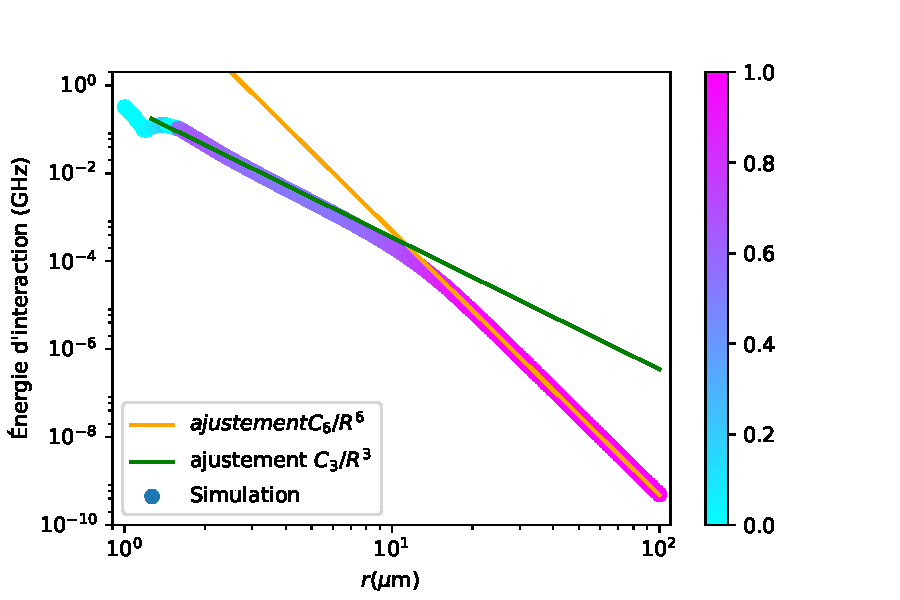
\includegraphics[width=1\linewidth]{figures/theory/VdW_50C50C_1Vcm}
\caption[Interaction dipolaire 50C-50C]{Déplacement en énergie de la paire 50C-50C placés côte à côte (cf fig\eqref{fig:double_torus}) par interaction dipolaire, sous un champ électrique de $\SIvv{1}{\V / \cm}$. L'échelle de couleur représente le carré de la projection sur l'état non perturbé $\ket{50\text{C},50\text{C}}$ de l'état propre du hamiltonien qui le suit adiabatiquement.
Le comportement dévie franchement de la forme de Van der Waals en $1/r^6$ dès que la distance interatomique est inférieure à $\SIv{10}{\micro\meter}$.
%Aux très courtes distances, le couplage vers d'autres niveaux atomiques devient très fort et l'énergie d'interaction}
}
\label{fig:VdW_50C50C_1Vcm}
\end{figure}

La figure \eqref{fig:VdW_50C50C_1Vcm} présente le résultat du calcul numérique.
Aux grandes distances, l'énergie d'interaction varie bien en $1/r^6$ comme on l'attend, avec un coefficient de Van der Waals 
\begin{equation}
\label{eq:C6_50C50C}
C_{6,50C50C}(\SIvv{1}{V/cm}) = \SIv{483.17}{\GHz\raiseto{6}\um}.
\end{equation}
Mais dès que les atomes se rapprochent à une distance inférieure à $\SIvv{10}{\um}$, l'énergie d'interaction varie en $1/r^3$ jusqu'à très courte distance.
En effet, lorsque l'interaction dipolaire devient suffisamment forte, le champ électrique extérieur ne suffit plus à définir le plan des orbites, et le niveau de paire est perturbé.
C'est ce que l'on retrouve sur la coloration de la courbe : à une distance critique de l'ordre de $\SIvv{10}{\um}$ le niveau de la paire s'éloigne du niveau non perturbé $\ket{\mathrm{50C,50C}}$.
La paire est alors dans un état superposé de plusieurs $\ket{nmk,n'm'k'}$, entre lesquels apparaissent des couplages dipolaires résonants en $1/r^3$.
Ce problème sera traité en détail dans le chapitre \ref{chapter:circsim}, lorsque nous nous intéresserons aux conditions dans lesquelles les interactions entre atomes circulaires sont les plus avantageuses pour la simulation quantique.

Si l'on approche encore les deux atomes, à des distances inférieures à \SIvv{2}{\um}, la base des états propres du hamiltonien de paire devient très différente de la base des états non perturbés.
Il est alors très difficile de décrire simplement l'interaction dipolaire.

\section*{Conclusion}
\noindent Nous avons dans ce chapitre présenté les caractéristiques physiques principales des atomes de Rydberg alcalins.
Nous avons utilisé la théorie du défaut quantique afin de décrire les niveaux de Rydberg de faible moment cinétique.
Ceux-ci dévient en effet du modèle de l'atome d'hydrogène par les effets de pénétration et de polarisabilité du c\oe ur atomique, ce que permet de corriger le défaut quantique.
Ainsi nous avons pu décrire le niveau 60S, en donnant la forme de sa fonction d'onde, sa taille et sa durée de vie radiative à différentes températures.

Nous nous sommes ensuite intéressés aux niveaux de Rydberg circulaires, qui semblent être de meilleurs candidats pour la simulation quantique grâce à leur temps de vie plus long.
La théorie du défaut quantique n'est plus nécessaire pour décrire les niveaux circulaires.
Cependant, l'introduction de la base des états paraboliques est d'une grande aide à leur description, en particulier en présence d'un champ électrique.
Nous avons ainsi pu décrire le niveau de Rydberg circulaire 50C, qui présente un temps de vie à température nulle de presque \SIvv{30}{\ms}.

En dernier lieu, nous avons vu comment les atomes de Rydberg interagissent entre eux par interaction dipolaire.
\`A grande distance, l'interaction dipolaire entre deux atomes de Rydberg prend la forme de Van der Waals avec une dépendance en $C_6/r^6$, où $r$ est la distance entre les deux atomes.
Nous avons pu déterminer les coefficients de Van der Waals $C_6$ pour l'interaction entre une paire d'atomes dans les niveaux $\ket{\text{60S,60S}}$, $\ket{\text{60S,nl}}$ et $\ket{\text{50C,50C}}$, en diagonalisant à chaque fois le hamiltonien complet du système pour toutes les distances $r$.
Aux distances très courtes, lorsque l'interaction dipolaire devient comparable aux différences d'énergie entre les niveaux de Rydberg, les niveaux de Rydberg se mélangent et l'interaction dipolaire ne peut plus être traitée simplement.

Les expériences que nous avons menées portent sur l'étude de l'interaction dipolaire entre atomes de Rydberg.
Il nous a fallu pour cela mettre en \oe uvre un dispositif expérimental que nous présentons dans le prochain chapitre.% \eqref{chapter:setup_coldatoms_Rydberg} .

%Plus particulièrement, nous avons étudié l'interaction dipolaire au sein d'un nuage dense d'atomes dans le niveau 60S, et nous avons 

%Les particularités de l'interaction dipolaire entre niveaux de très grand $l$ sera traitée au chapite \ref{chapter:circsim}.